\documentclass{article}

  % packages
    % basic stuff for rendering math
    \usepackage[letterpaper, top=1in, bottom=1in, left=1in, right=1in]{geometry}
    \usepackage[utf8]{inputenc}
    \usepackage[english]{babel}
    \usepackage{amsmath} 
    \usepackage{amssymb}
    \usepackage{bookmark}

    % extra math symbols and utilities
    \usepackage{mathtools}        % for extra stuff like \coloneqq
    \usepackage{mathrsfs}         % for extra stuff like \mathsrc{}
    \usepackage{centernot}        % for the centernot arrow 
    \usepackage{bm}               % for better boldsymbol/mathbf 
    \usepackage{enumitem}         % better control over enumerate, itemize
    \usepackage{hyperref}         % for hypertext linking
    \usepackage{xr-hyper}
    \usepackage{fancyvrb}          % for better verbatim environments
    \usepackage{newverbs}         % for texttt{}
    \usepackage{xcolor}           % for colored text 
    \usepackage{listings}         % to include code
    \usepackage{lstautogobble}    % helper package for code
    \usepackage{parcolumns}       % for side by side columns for two column code
    \usepackage{algorithm}
    \usepackage{algpseudocode}
    \usepackage{bbm}
    \algblock{Class}{EndClass}

    % page layout
    \usepackage{fancyhdr}         % for headers and footers 
    \usepackage{uniquecounter}
    \usepackage{lastpage}         % to include last page number in footer 
    \usepackage{parskip}          % for no indentation and space between paragraphs   
    \usepackage[T1]{fontenc}      % to include \textbackslash
    \usepackage{footnote}
    \usepackage{etoolbox}

    % for custom environments
    \usepackage{tcolorbox}        % for better colored boxes in custom environments
    \tcbuselibrary{breakable}     % to allow tcolorboxes to break across pages

    % figures
    \usepackage{pgfplots}
    \pgfplotsset{compat=1.18}
    \usepackage{float}            % for [H] figure placement
    \usepackage{tikz}
    \usepackage{tikz-cd}
    \usepackage{circuitikz}
    \usetikzlibrary{arrows, arrows.meta}
    \usetikzlibrary{positioning}
    \usetikzlibrary{calc}
    \usepackage{graphicx}
    \usepackage{caption} 
    \usepackage{subcaption}
    \captionsetup{font=small} 

    % for tabular stuff 
    \usepackage{dcolumn}

    \usepackage[nottoc]{tocbibind}
    \pdfsuppresswarningpagegroup=1
    \hfuzz=5.002pt                % ignore overfull hbox badness warnings below this limit

  % New and replaced operators
    \DeclareMathOperator{\Tr}{Tr}
    \DeclareMathOperator{\Sym}{Sym}
    \DeclareMathOperator{\Span}{span}
    \DeclareMathOperator{\elbo}{ELBO}
    \DeclareMathOperator{\std}{std}
    \DeclareMathOperator{\Cov}{Cov}
    \DeclareMathOperator{\Var}{Var}
    \DeclareMathOperator{\Corr}{Corr}
    \DeclareMathOperator{\pos}{pos}
    \DeclareMathOperator*{\argmin}{\arg\!\min}
    \DeclareMathOperator*{\argmax}{\arg\!\max}
    \newcommand{\qed}{\hfill$\blacksquare$}     % I like QED squares to be black

  % Custom Environments
    \newtcolorbox[auto counter, number within=section]{question}[1][]
    {
      colframe = orange!25,
      colback  = orange!10,
      coltitle = orange!20!black,  
      breakable, 
      title = \textbf{Question \thetcbcounter ~(#1)}
    }

    \newtcolorbox[auto counter, number within=section]{exercise}[1][]
    {
      colframe = teal!25,
      colback  = teal!10,
      coltitle = teal!20!black,  
      breakable, 
      title = \textbf{Exercise \thetcbcounter ~(#1)}
    }
    \newtcolorbox[auto counter, number within=section]{solution}[1][]
    {
      colframe = violet!25,
      colback  = violet!10,
      coltitle = violet!20!black,  
      breakable, 
      title = \textbf{Solution \thetcbcounter}
    }
    \newtcolorbox[auto counter, number within=section]{lemma}[1][]
    {
      colframe = red!25,
      colback  = red!10,
      coltitle = red!20!black,  
      breakable, 
      title = \textbf{Lemma \thetcbcounter ~(#1)}
    }
    \newtcolorbox[auto counter, number within=section]{theorem}[1][]
    {
      colframe = red!25,
      colback  = red!10,
      coltitle = red!20!black,  
      breakable, 
      title = \textbf{Theorem \thetcbcounter ~(#1)}
    } 
    \newtcolorbox[auto counter, number within=section]{corollary}[1][]
    {
      colframe = red!25,
      colback  = red!10,
      coltitle = red!20!black,  
      breakable, 
      title = \textbf{Corollary \thetcbcounter ~(#1)}
    } 
    \newtcolorbox[auto counter, number within=section]{proof}[1][]
    {
      colframe = orange!25,
      colback  = orange!10,
      coltitle = orange!20!black,  
      breakable, 
      title = \textbf{Proof. }
    } 
    \newtcolorbox[auto counter, number within=section]{definition}[1][]
    {
      colframe = yellow!25,
      colback  = yellow!10,
      coltitle = yellow!20!black,  
      breakable, 
      title = \textbf{Definition \thetcbcounter ~(#1)}
    } 
    \newtcolorbox[auto counter, number within=section]{example}[1][]
    {
      colframe = blue!25,
      colback  = blue!10,
      coltitle = blue!20!black,  
      breakable, 
      title = \textbf{Example \thetcbcounter ~(#1)}
    } 
    \newtcolorbox[auto counter, number within=section]{code}[1][]
    {
      colframe = green!25,
      colback  = green!10,
      coltitle = green!20!black,  
      breakable, 
      title = \textbf{Code \thetcbcounter ~(#1)}
    } 
    \newtcolorbox[auto counter, number within=section]{algo}[1][]
    {
      colframe = green!25,
      colback  = green!10,
      coltitle = green!20!black,  
      breakable, 
      title = \textbf{Algorithm \thetcbcounter ~(#1)}
    } 
    \definecolor{cverbbg}{gray}{0.93}
    \newenvironment{cverbatim}
      {\SaveVerbatim{cverb}}
      {\endSaveVerbatim
        \flushleft\fboxrule=0pt\fboxsep=.5em
        \colorbox{cverbbg}{%
          \makebox[\dimexpr\linewidth-2\fboxsep][l]{\BUseVerbatim{cverb}}%
        }
        \endflushleft
    }

    \definecolor{dkgreen}{rgb}{0,0.6,0}
    \definecolor{gray}{rgb}{0.5,0.5,0.5}
    \definecolor{mauve}{rgb}{0.58,0,0.82}
    \definecolor{lightgray}{gray}{0.93}
    \renewcommand{\algorithmiccomment}[1]{\hfill$\triangleright$\textcolor{blue}{#1}}

    % default options for listings (for code)
    \lstset{
      autogobble,
      frame=ltbr,
      language=Python,                           % the language of the code
      aboveskip=3mm,
      belowskip=3mm,
      showstringspaces=false,
      columns=fullflexible,
      keepspaces=true,
      basicstyle={\small\ttfamily},
      numbers=left,
      firstnumber=1,                        % start line number at 1
      numberstyle=\tiny\color{gray},
      keywordstyle=\color{blue},
      commentstyle=\color{dkgreen},
      stringstyle=\color{mauve},
      backgroundcolor=\color{lightgray}, 
      breaklines=true,                      % break lines
      breakatwhitespace=true,
      tabsize=3, 
      xleftmargin=2em, 
      framexleftmargin=1.5em, 
      stepnumber=1
    }

  % Page style
    \pagestyle{fancy}
    \fancyhead[L]{Encoder-Decoder Models}
    \fancyhead[C]{Muchang Bahng}
    \fancyhead[R]{Spring 2023} 
    \fancyfoot[C]{\thepage / \pageref{LastPage}}
    \renewcommand{\footrulewidth}{0.4pt}          % the footer line should be 0.4pt wide
    \renewcommand{\thispagestyle}[1]{}  % needed to include headers in title page
%    \renewcommand{\thefootnote}{\arabic{footnote}}

  % external documents 
    \externaldocument[algo-]{../../Computer_Science/DSA/paper}[../../Computer_Science/DSA/paper.pdf]

\begin{document}

\tikzset{every picture/.style={line width=0.75pt}} 

\title{Encoder-Decoder Models}
\author{Muchang Bahng}
\date{Spring 2023}

\maketitle
\tableofcontents
\pagebreak 

This covers computability theory, complexity theory, and automata theory. 
Alphabet. Boolean logic



\section{Encoder-Decoder Models}

  Encoder decoder models refer to a model consisting of two neural nets: the encoder that takes in the input and maps it to some lower-dimensional vector. Then, the decoder takes in this encoded vector and attempts to use it to decode what we're trying to get. The type of neural network can be any: MLP, CNN, or RNN, depending on what problem you're trying to achieve. 

  Now, why would we want to do something like encode the input into some lower dimensional setting, and then have the decoder neural net extract what we want? It seems like we're making the problem harder. There are two reasons: 
  \begin{enumerate}
    \item The input vector may not be in the correct form that we want. This is the motivation for the \textit{seq2seq} model, where we are working with sequences of vectors that suffer from the problem of \textit{locality} in RNNs. Therefore, it is necessary to encode this entire sequence into one vector, at the loss of dimension. 

    \item The input vector may be noisy or too high-dimensional itself. In CNNs, we saw that convolutional layers or pooling layers allow us to reduce the dimension to extract meaningful features from it. Likewise, we can train the encoder to extract useful features into a lower dimensional space, and then the decoder can efficiently work with this representation. This motivates the use of \textbf{autoencoders}, which can be done with MLPs, CNNs, or even RNNs. 
  \end{enumerate}

  Note that while these two algorithms fall in the paradigm of encoder-decoder networks, the seq2seq model is supervised while the autoencoder is unsupervised. In the seq2seq model, which deals with things like machine translation, we have a labeled dataset of sentences in language A corresponding with sentences in language B. However, in autoencoders, what we do is take a sample $x$ from our dataset and use it both as the input and output to train our network. Since there is no additional labeling required, this is an unsupervised learning technique. 

\subsection{Autoencoders}

  In the totally linear case, we have PCA. Some input $\mathbf{x} \in \mathcal{X} = \mathbb{R}^d$ is mapped to a smaller-dimensional $\mathcal{Z} = \mathbb{R}^k$. 
  \[\mathbf{x} \xlongrightarrow[]{V} \mathbf{z} \xlongrightarrow{U} \hat{\mathbf{x}}\]
  and so the ``network" essentially computes $\hat{\mathbf{x}} = U V \mathbf{x}$. Obviously the fact that $k < d$ is essential, since if $k \geq d$ then we can choose $U$ and $V$ such that $UV = I$, which is trivial. 

  This can be used for the following problem: Given $m$ points $\mathbf{x}_1, \ldots, \mathbf{x}_m \in \mathbb{R}^d$ and target dimension $k < d$, find the best $k$-dimensional subspade approximating the data. Formally, we want to find the matrices $U \in \mathbb{R}^{d \times k}$ and $V \in \mathbb{R}^{k \times d}$ that minimizes 
  \[f(U, V) = \sum_{i=1}^m ||\mathbf{x}_i - U V \mathbf{x}_i||_2^2 \] 
  where $V$ is the \textit{compressor} and $U$ is the \textit{decompressor}. Now unfortunately, this loss $f$ is not convex, though $f(U, \cdot)$ and $f(\cdot, V)$ are both convex. 

  \begin{theorem}
  We claim that the optimal solution is achieved when $U = V^T$ and $U^T U = I$. 
  \end{theorem}
  \begin{proof}
      For any $U, V$, the linear map $\mathbf{x} \mapsto U V \mathbf{x}$ has a range $R$ that forms a subspace of dimension $k$. Let $w_1, \ldots,w_k$ be an orthonormal basis for $R$, which we arrange into columns of $W$. Hence, for each $x_i$ there is $z_i \in \mathbb{R}^k$ such that $UV x_i = W z_i$. Note that by construction,$W^T W = I$. Now we want to find out which $z$ minimizes $f(x_i, z) = ||x_i - W z||_2^2$. We know that for all $x \in \mathbb{R}^d, z \in \mathbb{R}^k$, 
  \[f(x, z) = ||x||_2^2 + z^T W^T W z - 2 z^T W^T x = ||x||_2^2 + ||z||_2^2 - 2 z^T W^T x\] 
  We want to minimize w.r.t. to $z$, so by taking the derivative and setting to $0$, we get $z = W^T x$. This means that 
  \[\sum_{i=1}^m ||x_i - U V x_i ||^2 \geq \sum_{i=1}^m ||x_i - UV x_i||^2 \geq \sum_{i=1}^m ||x_i - W W^T x_i||^2\] 
  and since $U, V$ are optimal, equality is achieved and so instead of $U, V$, we can take $W, W^T$, with $W W^T x$ being the orthogonal projection of $x$ onto $R$. 
  \end{proof}

  One application of PCA is eigenfaces, which assumes that the set of all faces (projected onto an image) approximately lies in a hyperplane. 

  Autoencoders are a nonlinear generalization of PCA. We only use the inputs $\mathbf{x}_t$ for learning. We want to automatically extract meaningful features for the data and leverage the availability of unlabeled data. It can be used for visualization and compression. We can also build generative models with autoencoders. We can have several architectures, with none, one, or both the encoder/decoder having nonlinear activitation functions. Here is one architecture. 

  \begin{definition}[Autoencoder]
    An autoencoder is a feed-forward neural net whose job is to take an input $\mathbf{x}$ and output $\hat{\mathbf{x}}$. It consists of an encoder $E_\phi: \mathcal{X} \rightarrow \mathcal{Z}$ and decoder $D_\theta: \mathcal{Z} \rightarrow \mathcal{X}$, where $\mathcal{X}$ is the input/output space and $\mathcal{Z}$ is the latent feature space. 

    \begin{enumerate}
      \item The encoder model transforms $\mathbf{x}$ to a latent feature representation $\mathbf{z}$. It is a feed-foward, buttom-up neural net. 
      \item The decoder model maps $\mathbf{z}$ to a reconstruction $\hat{\mathbf{x}}$. It is generative, top-down. 
    \end{enumerate}
    where we have 
    \begin{align*} 
        \mathrm{Encoder} & : \mathbf{h}(\mathbf{x}) = g(\mathbf{a}(x)) = \sigma (\mathbf{b} + \mathbf{W} \mathbf{x}) \\
        \mathrm{Decoder} & : \hat{\mathbf{a}}(\mathbf{x}) = \sigma (\mathbf{c} + \mathbf{W}^\ast \mathbf{h}(\mathbf{x})) 
    \end{align*} 
    \begin{figure}[H]
      \centering 
      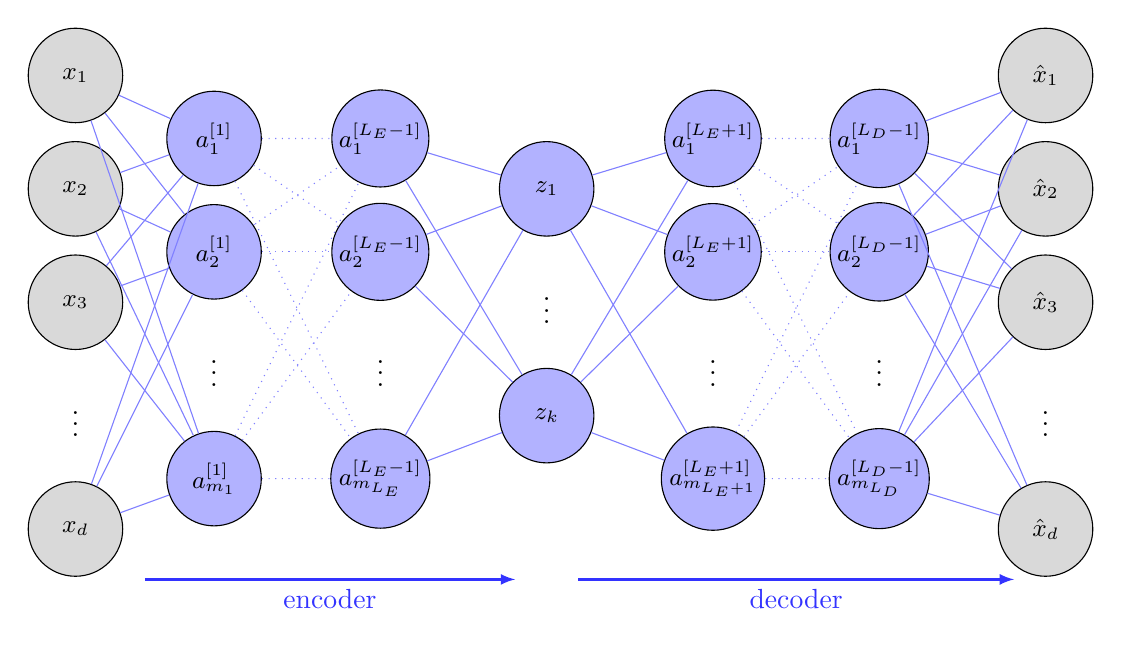
\begin{tikzpicture}[
          scale=0.8,
          node distance=2cm,
          neuron/.style={circle, draw, minimum size=1.2cm, inner sep=1.2pt, font=\small},
          annotation/.style={text width=3cm},
          >=latex
      ]
          % Define some variables for consistent spacing
          \def\layersep{2.2}
          \def\neuronsep{1.8}
          
          % Input layer (x)
          \node[neuron, fill=gray!30] (x1) at (0, 3) {$x_1$};
          \node[neuron, fill=gray!30] (x2) at (0, {3-\neuronsep}) {$x_2$};
          \node[neuron, fill=gray!30] (x3) at (0, {3-2*\neuronsep}) {$x_3$};
          \node at (0, {3-3*\neuronsep}) {$\vdots$};
          \node[neuron, fill=gray!30] (xd) at (0, {3-4*\neuronsep}) {$x_d$};
          
          % First hidden layer (encoder)
          \node[neuron, fill=blue!30] (a11) at (\layersep, 2) {$a^{[1]}_1$};
          \node[neuron, fill=blue!30] (a12) at (\layersep, {2-\neuronsep}) {$a^{[1]}_2$};
          \node at (\layersep, {2-2*\neuronsep}) {$\vdots$};
          \node[neuron, fill=blue!30] (a1m) at (\layersep, {2-3*\neuronsep}) {$a^{[1]}_{m_1}$};
          
          % Last encoder layer
          \node[neuron, fill=blue!30] (aE1) at (2.2*\layersep, 2) {$a^{[L_E-1]}_1$};
          \node[neuron, fill=blue!30] (aE2) at (2.2*\layersep, {2-\neuronsep}) {$a^{[L_E-1]}_2$};
          \node at (2.2*\layersep, {2-2*\neuronsep}) {$\vdots$};
          \node[neuron, fill=blue!30] (aEm) at (2.2*\layersep, {2-3*\neuronsep}) {$a^{[L_E-1]}_{m_{L_E}}$};
          
          % Bottleneck layer (z)
          \node[neuron, fill=blue!30] (z1) at (3.4*\layersep, {1.2-0*\neuronsep}) {$z_1$};
          \node at (3.4*\layersep, {1.2-\neuronsep}) {$\vdots$};
          \node[neuron, fill=blue!30] (zm) at (3.4*\layersep, {1.2-2*\neuronsep}) {$z_k$};
          
          % First decoder layer
          \node[neuron, fill=blue!30] (aD11) at (4.6*\layersep, 2) {$a^{[L_E+1]}_1$};
          \node[neuron, fill=blue!30] (aD12) at (4.6*\layersep, {2-\neuronsep}) {$a^{[L_E+1]}_2$};
          \node at (4.6*\layersep, {2-2*\neuronsep}) {$\vdots$};
          \node[neuron, fill=blue!30] (aD1m) at (4.6*\layersep, {2-3*\neuronsep}) {$a^{[L_E+1]}_{m_{L_E+1}}$};
          
          % Last hidden layer before output
          \node[neuron, fill=blue!30] (aL1) at (5.8*\layersep, 2) {$a^{[L_D-1]}_1$};
          \node[neuron, fill=blue!30] (aL2) at (5.8*\layersep, {2-\neuronsep}) {$a^{[L_D-1]}_2$};
          \node at (5.8*\layersep, {2-2*\neuronsep}) {$\vdots$};
          \node[neuron, fill=blue!30] (aLm) at (5.8*\layersep, {2-3*\neuronsep}) {$a^{[L_D-1]}_{m_{L_D}}$};
          
          % Output layer
          \node[neuron, fill=gray!30] (y1) at (7*\layersep, 3) {$\hat{x}_1$};
          \node[neuron, fill=gray!30] (y2) at (7*\layersep, {3-\neuronsep}) {$\hat{x}_2$};
          \node[neuron, fill=gray!30] (y3) at (7*\layersep, {3-2*\neuronsep}) {$\hat{x}_3$};
          \node at (7*\layersep, {3-3*\neuronsep}) {$\vdots$};
          \node[neuron, fill=gray!30] (yd) at (7*\layersep, {3-4*\neuronsep}) {$\hat{x}_d$};
          
          % Draw connections
          \begin{scope}[blue!50, thin]
            % Input to first hidden
            \foreach \i in {1,2,3,d} {
                \foreach \j in {1,2,m} {
                    \draw (x\i) -- (a1\j);
                }
            }
            
            % First hidden to last encoder layer
            \foreach \i in {1,2,m} {
                \foreach \j in {1,2,m} {
                    \draw[dotted] (a1\i) -- (aE\j);
                }
            }
            
            % Last encoder to bottleneck
            \foreach \i in {1,2,m} {
                \foreach \j in {1,m} {
                    \draw (aE\i) -- (z\j);
                }
            }
            
            % Bottleneck to first decoder
            \foreach \i in {1,m} {
                \foreach \j in {1,2,m} {
                    \draw (z\i) -- (aD1\j);
                }
            }
            
            % First decoder to last hidden
            \foreach \i in {1,2,m} {
                \foreach \j in {1,2,m} {
                    \draw[dotted] (aD1\i) -- (aL\j);
                }
            }
            
            % Last hidden to output
            \foreach \i in {1,2,m} {
                \foreach \j in {1,2,3,d} {
                    \draw (aL\i) -- (y\j);
                }
            }
          \end{scope}
          
          % Add encoder/decoder arrows
          \draw[->, blue!80, thick] (\layersep/2, -5) -- (3.4*\layersep-0.5, -5) 
              node[midway, below, text=blue!80] {encoder};
          \draw[->, blue!80, thick] (3.4*\layersep+0.5, -5) -- (7*\layersep-0.5, -5)
              node[midway, below, text=blue!80] {decoder};
      \end{tikzpicture}
      \caption{A graphical model of an autoencoder. The $z$ is called the \textbf{bottleneck layer}, which compresses the input into a lower-dimensional representation. The $x$ is known as the \textbf{input layer}, the $\hat{x}$ as the \textbf{output layer}, and everything else are \textbf{hidden layers}.} 
      \label{fig:autoencoder}
    \end{figure}
  \end{definition}


  The parameter gradients are obtained by backpropagating the gradient $\nabla_{\theta} \mathcal{L}$ like a regular network, but if we force tied weights (i.e. $W^\ast = W^T$), then $\nabla_{\mathbf{W}} \mathcal{L}$ is the sum of two gradients. This is because $\mathbf{W}$ is present both in the encoder and decoder. 

  I want to train the whole neural network such that the error between $\mathbf{x}$ and $\hat{\mathbf{x}}$ is minimized. We can consider a squared-error, for example. 
  \begin{equation}
    \mathcal{L}(\mathbf{x}, \hat{\mathbf{x}}) = \frac{1}{2} ||\mathbf{x} - \hat{\mathbf{x}}||_2^2
  \end{equation}

  \begin{algo}
    An implementation of an autoencoder in PyTorch is \href{code/autoencoder.html}{here}. 
  \end{algo}

  There are three things we can do to extract meaningful hidden features: 
  \begin{enumerate}
    \item \textbf{Undercomplete Representation}: Make the latent dimension small. It compresses the input, but it may only be good for the training distribution and may not be robust to other types of input. If it is overcomplete, there is no guarantee that we will extract meaningful features. 

    \item \textbf{Denoising Autoencoder}: Injecting noise to the input. The idea is that the representation should be robust to the introduction of noise. We take the original input $\mathbf{x}$ and we randomly assign a subset of the inputs to $0$, with probability $\nu$, similar to dropout, to get our noisy input $\Tilde{\mathbf{x}}$. Then we train the autoencoder with the loss comparing the output $\hat{\mathbf{x}}$ to the original, un-noisy input $\mathbf{x}$. We can do this for Gaussian additive noise too. As the visual below suggests, we are essentially ``pushing" out inputs away from the manifold and training the autoencoder to denoise it, pulling it back. 

      \begin{center}
          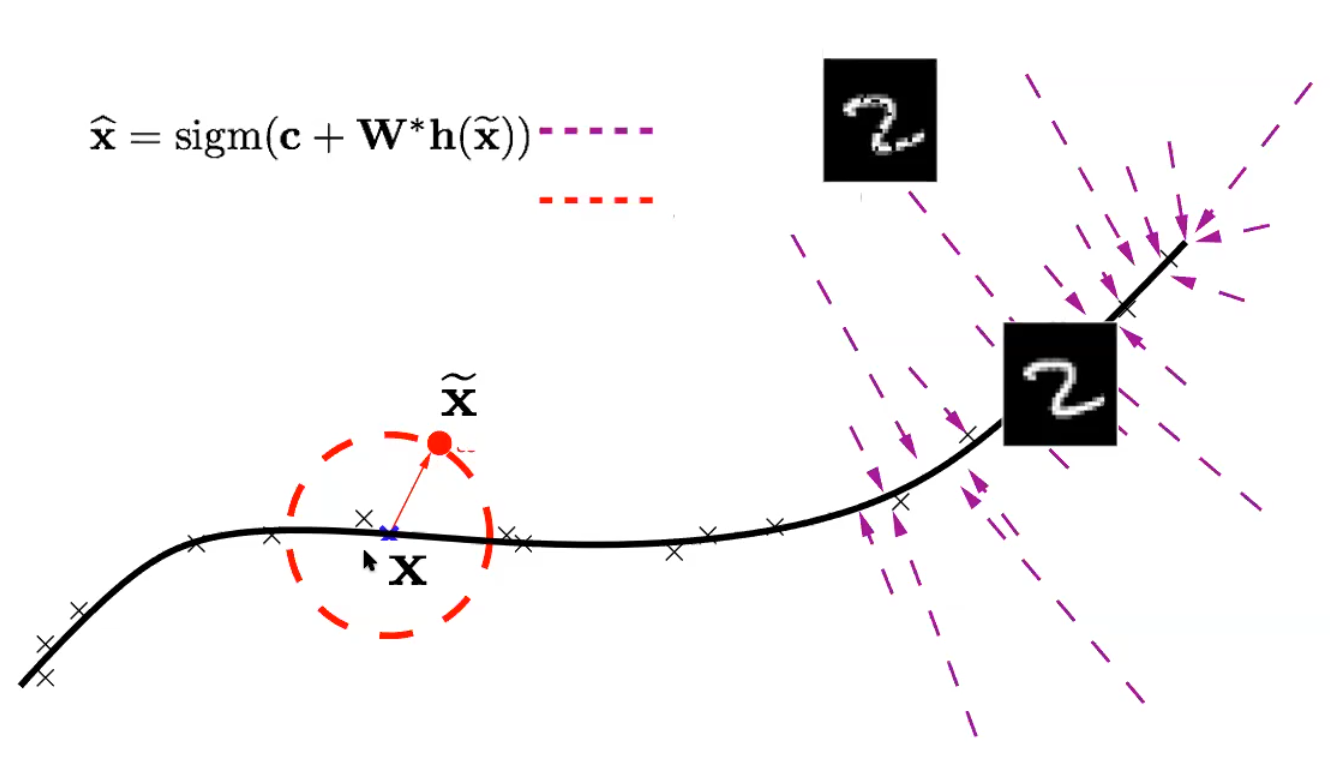
\includegraphics[scale=0.3]{img/denoising_autoencoder.png}
      \end{center}
  
    \item \textbf{Contractive Autoencoder}: If we have the latent dimension greater than the input, then we can just add an explict term in the loss that penalizes that solution (e.g. promoting sparsity). For example, we can have the loss be 
    \[\mathcal{L}(f(\mathbf{x}^{(t)}) + \lambda || \nabla_{\mathbf{x}^{(t)}} \mathbf{h}(\mathbf{x}^{(t)})||^2_F\]
    where 
    \[||\nabla_{\mathbf{x}^{(t)}} \mathbf{h}(\mathbf{x}^{(t)})||_F^2 = \sum_{j, k} \bigg(\frac{\partial h(\mathbf{x}^{(t)})_j}{\partial x_k^{(t)}} \bigg)^2\]
    which forces the encoder to throw away information. If one of the elements are $0$, then we know that the $k$th element of the input has no effect on the $j$th element of the encoded output. Therefore, it tries to throw away as many elements of $\mathbf{x}$ as possible since the identity matrix will have a large Frobenius norm, essentially contracting the input representation.  

    We can also promote sparsity by adding a L1 penalty, forcing the feature space to be sparse. 
  \end{enumerate}

  The \textbf{predictive sparse decomposition} shows that the loss should be 
  \begin{equation}
    \min_{W, W^\ast, \mathbf{z}} ||W^\ast \mathbf{z} - \mathbf{x}||^2_2 + \lambda | \mathbf{z}|_1 + ||\sigma(W \mathbf{x}) - \mathbf{z}||^2_2
  \end{equation}
  where the first term tells the decoder to reconstruct the original input well, the second tells the latent vector to be sparse, and the third tells us that we shouldn't lose too much information when we encode. 

  We could also have \textbf{stacked autoencoders}, with each layer of latent features having some desired sparsity. 

\subsection{Sequence to Sequence}

  We have mentioned that RNNs and LSTMs have the advantage of mapping from variable length inputs to variable length outputs. This can be done for any length input and any length output. However, the RNN has the problem of \textit{locality}, that the words next to the current word have a greater effect, and we are trying to generate sequences on the fly by reading in each word. Even for bidirectional RNNs, where we go through the whole sentence first, the effects of adjacent words have a greater effect when generating outputs. It would be wiser to read the \textit{whole} sentence and then start to generate a sequence. This is the motivation for the \textbf{encoder-decoder model}. It is conventionally divided into a two-stage network. 
  \begin{enumerate}
    \item The encoder neural net would convert a sequence into a single latent space representation $z = f(x)$. This latent representation $z$ essentially refers to a feature (vector) representation, which is able to capture the underlying semantic information of the input that is useful for predicting the output. 
    \item The decoder neural net would decode this feature vector, called the \textbf{context vector}, into a sequence of the desired output $y = g(z)$ by using it as the initial hidden state. It uses the previous output as the next input for decoding. 
  \end{enumerate}
  Note that the encoder and decoder are two completely separate neural networks with their own parameters. This is important, since the fact that these are two completely separate networks allows us to work in different ``paradigms" within either the feature or target space. For example, if we want to perform machine translation from English to Spanish, our encoder RNN parameters have been tuned to the English syntax and language, while the decoder RNN parameters are tuned to the Spanish language. Since we are modeling different languages, it makes sense to have different sequence models for each one. 

  We will talk about a specific type of encoder-decoder model called \textbf{seq2seq}, which maps sequences to sequences using RNN encoders and decoders. Conventionally, the hidden nodes of the encoder are denoted with $\mathbf{h}$, and those of the decoder are denoted with $\mathbf{s}$. 
  \begin{enumerate}
      \item For the encoder, we take in the inputs $\mathbf{x}_t$ and generate the hidden states as 
      \begin{equation}
        \mathbf{h}_t = f(\mathbf{x}_t, \mathbf{h}_{t-1}) = \mathbf{W}_e \mathbf{h}_{t-1} + \mathbf{U}_e \mathbf{x}_t + \mathbf{b}_e
      \end{equation}
      In general, the encoder transforms the hidden states at all time steps into a context variable through the composition of functions $q$ 
      \[\mathbf{C} = q(\mathbf{h}_1, \mathbf{h}_2, \ldots, \mathbf{h}_T)\]
      In the figure below, the context variable is just $\mathbf{C} = \mathbf{h}_T$. 

      \item Now, given the target output sequence $\hat{\mathbf{y}}_1, \ldots, \hat{\mathbf{y}}_{t^\prime + 1}$ for each timestep $t^\prime$ (we use $t^\prime$ to differentiate from the input sequence time steps), the decoder assigns a predicted probability to each possible token occurring at step $\hat{\mathbf{y}}_{t^\prime + 1}$ conditioned on both the previous tokens $\hat{\mathbf{y}}_1, \ldots, \hat{\mathbf{y}}_{t^\prime + 1}$ and the context variable $\mathbf{C}$, i.e. 
      \[\mathbb{P}(\hat{\mathbf{y}}_{t^\prime + 1} \mid \hat{\mathbf{y}}_1, \ldots, \hat{\mathbf{y}}_{t^\prime + 1}, \mathbf{C})\]
      Therefore, to decode the subsequent token $\hat{\mathbf{y}}_{t^\prime + 1}$, we calculate the hidden state $\mathbf{s}_{t^\prime + 1}$ as a gated hidden unit computed by 
      \[\mathbf{s}_{t^\prime + 1} = g(\mathbf{s}_{t^\prime}, \hat{\mathbf{y}}_{t^\prime}, \mathbf{C})\]
      with the math mentioned \href{https://arxiv.org/pdf/1409.0473.pdf#page=12}{here}. 
  \end{enumerate}

  \begin{figure}[H]
    \centering 
    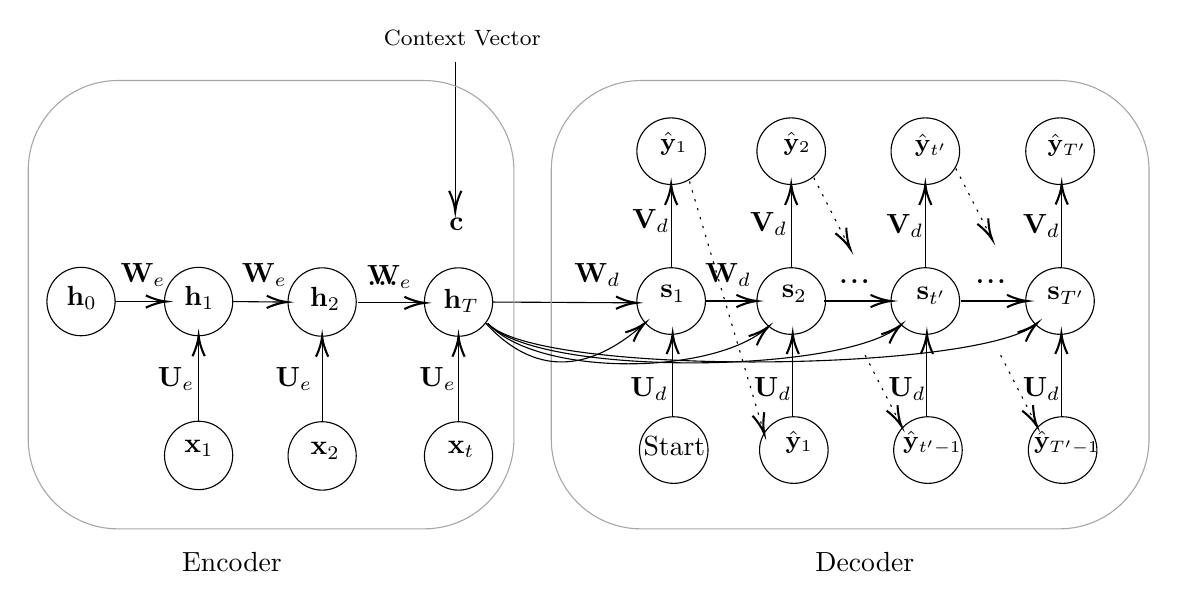
\begin{tikzpicture}[x=0.75pt,y=0.75pt,yscale=-0.9,xscale=0.9]
      %Shape: Ellipse [id:dp12104572681386716] 
      \draw   (169.09,148.58) .. controls (169.09,138.47) and (177.26,130.27) .. (187.34,130.27) .. controls (197.42,130.27) and (205.59,138.47) .. (205.59,148.58) .. controls (205.59,158.69) and (197.42,166.89) .. (187.34,166.89) .. controls (177.26,166.89) and (169.09,158.69) .. (169.09,148.58) -- cycle ;
      %Shape: Ellipse [id:dp741120269708732] 
      \draw   (242.1,148.58) .. controls (242.1,138.47) and (250.27,130.27) .. (260.35,130.27) .. controls (270.43,130.27) and (278.6,138.47) .. (278.6,148.58) .. controls (278.6,158.69) and (270.43,166.89) .. (260.35,166.89) .. controls (250.27,166.89) and (242.1,158.69) .. (242.1,148.58) -- cycle ;
      %Shape: Ellipse [id:dp42031301232731244] 
      \draw   (102.96,148.31) .. controls (102.96,138.2) and (111.14,130) .. (121.22,130) .. controls (131.29,130) and (139.47,138.2) .. (139.47,148.31) .. controls (139.47,158.42) and (131.29,166.62) .. (121.22,166.62) .. controls (111.14,166.62) and (102.96,158.42) .. (102.96,148.31) -- cycle ;
      %Shape: Ellipse [id:dp04610349626863375] 
      \draw   (169.09,230.97) .. controls (169.09,220.86) and (177.26,212.66) .. (187.34,212.66) .. controls (197.42,212.66) and (205.59,220.86) .. (205.59,230.97) .. controls (205.59,241.08) and (197.42,249.28) .. (187.34,249.28) .. controls (177.26,249.28) and (169.09,241.08) .. (169.09,230.97) -- cycle ;
      %Shape: Ellipse [id:dp7588227428266139] 
      \draw   (242.1,230.97) .. controls (242.1,220.86) and (250.27,212.66) .. (260.35,212.66) .. controls (270.43,212.66) and (278.6,220.86) .. (278.6,230.97) .. controls (278.6,241.08) and (270.43,249.28) .. (260.35,249.28) .. controls (250.27,249.28) and (242.1,241.08) .. (242.1,230.97) -- cycle ;
      %Shape: Ellipse [id:dp3672959591373348] 
      \draw   (102.96,230.7) .. controls (102.96,220.59) and (111.14,212.39) .. (121.22,212.39) .. controls (131.29,212.39) and (139.47,220.59) .. (139.47,230.7) .. controls (139.47,240.81) and (131.29,249.01) .. (121.22,249.01) .. controls (111.14,249.01) and (102.96,240.81) .. (102.96,230.7) -- cycle ;
      %Straight Lines [id:da21018477228753185] 
      \draw [color={rgb, 255:red, 0; green, 0; blue, 0 }  ,draw opacity=1 ]   (121.22,212.39) -- (121.22,168.62) ;
      \draw [shift={(121.22,166.62)}, rotate = 90] [color={rgb, 255:red, 0; green, 0; blue, 0 }  ,draw opacity=1 ][line width=0.75]    (10.93,-3.29) .. controls (6.95,-1.4) and (3.31,-0.3) .. (0,0) .. controls (3.31,0.3) and (6.95,1.4) .. (10.93,3.29)   ;
      %Straight Lines [id:da17363282179045836] 
      \draw [color={rgb, 255:red, 0; green, 0; blue, 0 }  ,draw opacity=1 ]   (187.34,212.66) -- (187.34,168.89) ;
      \draw [shift={(187.34,166.89)}, rotate = 90] [color={rgb, 255:red, 0; green, 0; blue, 0 }  ,draw opacity=1 ][line width=0.75]    (10.93,-3.29) .. controls (6.95,-1.4) and (3.31,-0.3) .. (0,0) .. controls (3.31,0.3) and (6.95,1.4) .. (10.93,3.29)   ;
      %Straight Lines [id:da40218372998636487] 
      \draw [color={rgb, 255:red, 0; green, 0; blue, 0 }  ,draw opacity=1 ]   (260.35,212.66) -- (260.35,168.89) ;
      \draw [shift={(260.35,166.89)}, rotate = 90] [color={rgb, 255:red, 0; green, 0; blue, 0 }  ,draw opacity=1 ][line width=0.75]    (10.93,-3.29) .. controls (6.95,-1.4) and (3.31,-0.3) .. (0,0) .. controls (3.31,0.3) and (6.95,1.4) .. (10.93,3.29)   ;
      %Shape: Ellipse [id:dp9751332219640756] 
      \draw   (40,148.31) .. controls (40,138.2) and (48.17,130) .. (58.25,130) .. controls (68.33,130) and (76.5,138.2) .. (76.5,148.31) .. controls (76.5,158.42) and (68.33,166.62) .. (58.25,166.62) .. controls (48.17,166.62) and (40,158.42) .. (40,148.31) -- cycle ;
      %Straight Lines [id:da988218839650463] 
      \draw [color={rgb, 255:red, 0; green, 0; blue, 0 }  ,draw opacity=1 ]   (76.5,148.31) -- (101.88,148.31) ;
      \draw [shift={(103.88,148.31)}, rotate = 180] [color={rgb, 255:red, 0; green, 0; blue, 0 }  ,draw opacity=1 ][line width=0.75]    (10.93,-3.29) .. controls (6.95,-1.4) and (3.31,-0.3) .. (0,0) .. controls (3.31,0.3) and (6.95,1.4) .. (10.93,3.29)   ;
      %Straight Lines [id:da8149363438054458] 
      \draw [color={rgb, 255:red, 0; green, 0; blue, 0 }  ,draw opacity=1 ]   (139.47,148.31) -- (166.6,148.59) ;
      \draw [shift={(168.6,148.61)}, rotate = 180.59] [color={rgb, 255:red, 0; green, 0; blue, 0 }  ,draw opacity=1 ][line width=0.75]    (10.93,-3.29) .. controls (6.95,-1.4) and (3.31,-0.3) .. (0,0) .. controls (3.31,0.3) and (6.95,1.4) .. (10.93,3.29)   ;
      %Shape: Ellipse [id:dp8769921800297902] 
      \draw   (420.09,67.83) .. controls (420.09,57.98) and (428.31,50) .. (438.44,50) .. controls (448.58,50) and (456.79,57.98) .. (456.79,67.83) .. controls (456.79,77.67) and (448.58,85.65) .. (438.44,85.65) .. controls (428.31,85.65) and (420.09,77.67) .. (420.09,67.83) -- cycle ;
      %Shape: Ellipse [id:dp8525299588463036] 
      \draw   (491.9,67.83) .. controls (491.9,57.98) and (500.11,50) .. (510.25,50) .. controls (520.38,50) and (528.6,57.98) .. (528.6,67.83) .. controls (528.6,77.67) and (520.38,85.65) .. (510.25,85.65) .. controls (500.11,85.65) and (491.9,77.67) .. (491.9,67.83) -- cycle ;
      %Shape: Ellipse [id:dp09036435821311728] 
      \draw   (420.09,148.04) .. controls (420.09,138.2) and (428.31,130.21) .. (438.44,130.21) .. controls (448.58,130.21) and (456.79,138.2) .. (456.79,148.04) .. controls (456.79,157.88) and (448.58,165.87) .. (438.44,165.87) .. controls (428.31,165.87) and (420.09,157.88) .. (420.09,148.04) -- cycle ;
      %Shape: Ellipse [id:dp23880588274822712] 
      \draw   (491.9,148.04) .. controls (491.9,138.2) and (500.11,130.21) .. (510.25,130.21) .. controls (520.38,130.21) and (528.6,138.2) .. (528.6,148.04) .. controls (528.6,157.88) and (520.38,165.87) .. (510.25,165.87) .. controls (500.11,165.87) and (491.9,157.88) .. (491.9,148.04) -- cycle ;
      %Shape: Ellipse [id:dp4615954589889102] 
      \draw   (355.82,148.04) .. controls (355.82,138.2) and (364.04,130.21) .. (374.17,130.21) .. controls (384.3,130.21) and (392.52,138.2) .. (392.52,148.04) .. controls (392.52,157.88) and (384.3,165.87) .. (374.17,165.87) .. controls (364.04,165.87) and (355.82,157.88) .. (355.82,148.04) -- cycle ;
      %Straight Lines [id:da8663141237622789] 
      \draw [color={rgb, 255:red, 0; green, 0; blue, 0 }  ,draw opacity=1 ]   (392.52,148.04) -- (418.05,148.04) ;
      \draw [shift={(420.05,148.04)}, rotate = 180] [color={rgb, 255:red, 0; green, 0; blue, 0 }  ,draw opacity=1 ][line width=0.75]    (10.93,-3.29) .. controls (6.95,-1.4) and (3.31,-0.3) .. (0,0) .. controls (3.31,0.3) and (6.95,1.4) .. (10.93,3.29)   ;
      %Straight Lines [id:da054789319283937044] 
      \draw [color={rgb, 255:red, 0; green, 0; blue, 0 }  ,draw opacity=1 ]   (456.2,148.04) -- (489.9,148.04) ;
      \draw [shift={(491.9,148.04)}, rotate = 180] [color={rgb, 255:red, 0; green, 0; blue, 0 }  ,draw opacity=1 ][line width=0.75]    (10.93,-3.29) .. controls (6.95,-1.4) and (3.31,-0.3) .. (0,0) .. controls (3.31,0.3) and (6.95,1.4) .. (10.93,3.29)   ;
      %Straight Lines [id:da8426206211081082] 
      \draw [color={rgb, 255:red, 0; green, 0; blue, 0 }  ,draw opacity=1 ]   (438.44,130.21) -- (438.44,87.65) ;
      \draw [shift={(438.44,85.65)}, rotate = 90] [color={rgb, 255:red, 0; green, 0; blue, 0 }  ,draw opacity=1 ][line width=0.75]    (10.93,-3.29) .. controls (6.95,-1.4) and (3.31,-0.3) .. (0,0) .. controls (3.31,0.3) and (6.95,1.4) .. (10.93,3.29)   ;
      %Straight Lines [id:da11805221789762355] 
      \draw [color={rgb, 255:red, 0; green, 0; blue, 0 }  ,draw opacity=1 ]   (510.25,130.21) -- (510.25,99.91) -- (510.25,87.65) ;
      \draw [shift={(510.25,85.65)}, rotate = 90] [color={rgb, 255:red, 0; green, 0; blue, 0 }  ,draw opacity=1 ][line width=0.75]    (10.93,-3.29) .. controls (6.95,-1.4) and (3.31,-0.3) .. (0,0) .. controls (3.31,0.3) and (6.95,1.4) .. (10.93,3.29)   ;
      %Shape: Ellipse [id:dp22353660348109727] 
      \draw   (355.82,67.83) .. controls (355.82,57.98) and (364.04,50) .. (374.17,50) .. controls (384.3,50) and (392.52,57.98) .. (392.52,67.83) .. controls (392.52,77.67) and (384.3,85.65) .. (374.17,85.65) .. controls (364.04,85.65) and (355.82,77.67) .. (355.82,67.83) -- cycle ;
      %Straight Lines [id:da15189468948594165] 
      \draw [color={rgb, 255:red, 0; green, 0; blue, 0 }  ,draw opacity=1 ]   (374.17,130.21) -- (374.17,99.91) -- (374.17,87.65) ;
      \draw [shift={(374.17,85.65)}, rotate = 90] [color={rgb, 255:red, 0; green, 0; blue, 0 }  ,draw opacity=1 ][line width=0.75]    (10.93,-3.29) .. controls (6.95,-1.4) and (3.31,-0.3) .. (0,0) .. controls (3.31,0.3) and (6.95,1.4) .. (10.93,3.29)   ;
      %Straight Lines [id:da7646592734808089] 
      \draw [color={rgb, 255:red, 0; green, 0; blue, 0 }  ,draw opacity=1 ]   (206.6,149.04) -- (240.3,149.04) ;
      \draw [shift={(242.3,149.04)}, rotate = 180] [color={rgb, 255:red, 0; green, 0; blue, 0 }  ,draw opacity=1 ][line width=0.75]    (10.93,-3.29) .. controls (6.95,-1.4) and (3.31,-0.3) .. (0,0) .. controls (3.31,0.3) and (6.95,1.4) .. (10.93,3.29)   ;
      %Straight Lines [id:da7609105327490961] 
      \draw    (258.6,20) -- (258.6,98) ;
      \draw [shift={(258.6,100)}, rotate = 270] [color={rgb, 255:red, 0; green, 0; blue, 0 }  ][line width=0.75]    (10.93,-3.29) .. controls (6.95,-1.4) and (3.31,-0.3) .. (0,0) .. controls (3.31,0.3) and (6.95,1.4) .. (10.93,3.29)   ;
      %Straight Lines [id:da815869668900407] 
      \draw [color={rgb, 255:red, 0; green, 0; blue, 0 }  ,draw opacity=1 ]   (278.6,148.58) -- (353.6,148.99) ;
      \draw [shift={(355.6,149)}, rotate = 180.31] [color={rgb, 255:red, 0; green, 0; blue, 0 }  ,draw opacity=1 ][line width=0.75]    (10.93,-3.29) .. controls (6.95,-1.4) and (3.31,-0.3) .. (0,0) .. controls (3.31,0.3) and (6.95,1.4) .. (10.93,3.29)   ;
      %Rounded Rect [id:dp8974917713272867] 
      \draw  [color={rgb, 255:red, 167; green, 167; blue, 167 }  ,draw opacity=1 ] (30,78) .. controls (30,51.49) and (51.49,30) .. (78,30) -- (242,30) .. controls (268.51,30) and (290,51.49) .. (290,78) -- (290,222) .. controls (290,248.51) and (268.51,270) .. (242,270) -- (78,270) .. controls (51.49,270) and (30,248.51) .. (30,222) -- cycle ;
      %Rounded Rect [id:dp621652359446494] 
      \draw  [color={rgb, 255:red, 167; green, 167; blue, 167 }  ,draw opacity=1 ] (310,78) .. controls (310,51.49) and (331.49,30) .. (358,30) -- (582,30) .. controls (608.51,30) and (630,51.49) .. (630,78) -- (630,222) .. controls (630,248.51) and (608.51,270) .. (582,270) -- (358,270) .. controls (331.49,270) and (310,248.51) .. (310,222) -- cycle ;
      %Straight Lines [id:da2968728075840934] 
      \draw [color={rgb, 255:red, 0; green, 0; blue, 0 }  ,draw opacity=1 ]   (439.27,210) -- (439.27,167.44) ;
      \draw [shift={(439.27,165.44)}, rotate = 90] [color={rgb, 255:red, 0; green, 0; blue, 0 }  ,draw opacity=1 ][line width=0.75]    (10.93,-3.29) .. controls (6.95,-1.4) and (3.31,-0.3) .. (0,0) .. controls (3.31,0.3) and (6.95,1.4) .. (10.93,3.29)   ;
      %Straight Lines [id:da38515939024710244] 
      \draw [color={rgb, 255:red, 0; green, 0; blue, 0 }  ,draw opacity=1 ]   (511.08,210) -- (511.08,179.7) -- (511.08,167.44) ;
      \draw [shift={(511.08,165.44)}, rotate = 90] [color={rgb, 255:red, 0; green, 0; blue, 0 }  ,draw opacity=1 ][line width=0.75]    (10.93,-3.29) .. controls (6.95,-1.4) and (3.31,-0.3) .. (0,0) .. controls (3.31,0.3) and (6.95,1.4) .. (10.93,3.29)   ;
      %Straight Lines [id:da14741802814240956] 
      \draw [color={rgb, 255:red, 0; green, 0; blue, 0 }  ,draw opacity=1 ]   (375,210) -- (375,193.6) -- (375,179.7) -- (375,167.44) ;
      \draw [shift={(375,165.44)}, rotate = 90] [color={rgb, 255:red, 0; green, 0; blue, 0 }  ,draw opacity=1 ][line width=0.75]    (10.93,-3.29) .. controls (6.95,-1.4) and (3.31,-0.3) .. (0,0) .. controls (3.31,0.3) and (6.95,1.4) .. (10.93,3.29)   ;
      %Shape: Ellipse [id:dp7615118627097319] 
      \draw   (421.5,227.83) .. controls (421.5,217.98) and (429.71,210) .. (439.85,210) .. controls (449.98,210) and (458.2,217.98) .. (458.2,227.83) .. controls (458.2,237.67) and (449.98,245.65) .. (439.85,245.65) .. controls (429.71,245.65) and (421.5,237.67) .. (421.5,227.83) -- cycle ;
      %Shape: Ellipse [id:dp640367209409753] 
      \draw   (493.3,227.83) .. controls (493.3,217.98) and (501.52,210) .. (511.65,210) .. controls (521.78,210) and (530,217.98) .. (530,227.83) .. controls (530,237.67) and (521.78,245.65) .. (511.65,245.65) .. controls (501.52,245.65) and (493.3,237.67) .. (493.3,227.83) -- cycle ;
      %Shape: Ellipse [id:dp18357530976130754] 
      \draw   (357.22,227.83) .. controls (357.22,217.98) and (365.44,210) .. (375.57,210) .. controls (385.71,210) and (393.92,217.98) .. (393.92,227.83) .. controls (393.92,237.67) and (385.71,245.65) .. (375.57,245.65) .. controls (365.44,245.65) and (357.22,237.67) .. (357.22,227.83) -- cycle ;
      %Straight Lines [id:da039581984918104274] 
      \draw  [dash pattern={on 0.84pt off 2.51pt}]  (384,84) -- (423.43,217.08) ;
      \draw [shift={(424,219)}, rotate = 253.5] [color={rgb, 255:red, 0; green, 0; blue, 0 }  ][line width=0.75]    (10.93,-3.29) .. controls (6.95,-1.4) and (3.31,-0.3) .. (0,0) .. controls (3.31,0.3) and (6.95,1.4) .. (10.93,3.29)   ;
      %Straight Lines [id:da6000754918163929] 
      \draw  [dash pattern={on 0.84pt off 2.51pt}]  (450.55,82.04) -- (469.09,118.22) ;
      \draw [shift={(470,120)}, rotate = 242.87] [color={rgb, 255:red, 0; green, 0; blue, 0 }  ][line width=0.75]    (10.93,-3.29) .. controls (6.95,-1.4) and (3.31,-0.3) .. (0,0) .. controls (3.31,0.3) and (6.95,1.4) .. (10.93,3.29)   ;
      %Straight Lines [id:da5632246037194519] 
      \draw [color={rgb, 255:red, 0; green, 0; blue, 0 }  ,draw opacity=1 ]   (529.2,148.04) -- (562.9,148.04) ;
      \draw [shift={(564.9,148.04)}, rotate = 180] [color={rgb, 255:red, 0; green, 0; blue, 0 }  ,draw opacity=1 ][line width=0.75]    (10.93,-3.29) .. controls (6.95,-1.4) and (3.31,-0.3) .. (0,0) .. controls (3.31,0.3) and (6.95,1.4) .. (10.93,3.29)   ;
      %Straight Lines [id:da564576595545853] 
      \draw  [dash pattern={on 0.84pt off 2.51pt}]  (478,177) -- (496.54,213.18) ;
      \draw [shift={(497.45,214.96)}, rotate = 242.87] [color={rgb, 255:red, 0; green, 0; blue, 0 }  ][line width=0.75]    (10.93,-3.29) .. controls (6.95,-1.4) and (3.31,-0.3) .. (0,0) .. controls (3.31,0.3) and (6.95,1.4) .. (10.93,3.29)   ;
      %Straight Lines [id:da2885206646010938] 
      \draw  [dash pattern={on 0.84pt off 2.51pt}]  (526.55,77.04) -- (545.09,113.22) ;
      \draw [shift={(546,115)}, rotate = 242.87] [color={rgb, 255:red, 0; green, 0; blue, 0 }  ][line width=0.75]    (10.93,-3.29) .. controls (6.95,-1.4) and (3.31,-0.3) .. (0,0) .. controls (3.31,0.3) and (6.95,1.4) .. (10.93,3.29)   ;
      %Curve Lines [id:da21184366007833177] 
      \draw    (275,160) .. controls (301.1,188.26) and (329.62,186.42) .. (358.67,161.17) ;
      \draw [shift={(360,160)}, rotate = 138.23] [color={rgb, 255:red, 0; green, 0; blue, 0 }  ][line width=0.75]    (10.93,-3.29) .. controls (6.95,-1.4) and (3.31,-0.3) .. (0,0) .. controls (3.31,0.3) and (6.95,1.4) .. (10.93,3.29)   ;
      %Curve Lines [id:da7156893211463737] 
      \draw    (276,160) .. controls (302.1,188.26) and (393.69,188.36) .. (424.63,163.17) ;
      \draw [shift={(426,162)}, rotate = 138.23] [color={rgb, 255:red, 0; green, 0; blue, 0 }  ][line width=0.75]    (10.93,-3.29) .. controls (6.95,-1.4) and (3.31,-0.3) .. (0,0) .. controls (3.31,0.3) and (6.95,1.4) .. (10.93,3.29)   ;
      %Curve Lines [id:da8926144138863956] 
      \draw    (276,160) .. controls (302.1,188.26) and (462.57,187.39) .. (495.58,162.17) ;
      \draw [shift={(497,161)}, rotate = 138.23] [color={rgb, 255:red, 0; green, 0; blue, 0 }  ][line width=0.75]    (10.93,-3.29) .. controls (6.95,-1.4) and (3.31,-0.3) .. (0,0) .. controls (3.31,0.3) and (6.95,1.4) .. (10.93,3.29)   ;
      %Shape: Ellipse [id:dp13692419886270235] 
      \draw   (564,67.83) .. controls (564,57.98) and (572.22,50) .. (582.35,50) .. controls (592.48,50) and (600.7,57.98) .. (600.7,67.83) .. controls (600.7,77.67) and (592.48,85.65) .. (582.35,85.65) .. controls (572.22,85.65) and (564,77.67) .. (564,67.83) -- cycle ;
      %Shape: Ellipse [id:dp3366510546944117] 
      \draw   (564,148.04) .. controls (564,138.2) and (572.22,130.21) .. (582.35,130.21) .. controls (592.48,130.21) and (600.7,138.2) .. (600.7,148.04) .. controls (600.7,157.88) and (592.48,165.87) .. (582.35,165.87) .. controls (572.22,165.87) and (564,157.88) .. (564,148.04) -- cycle ;
      %Shape: Ellipse [id:dp8287297044956745] 
      \draw   (565.4,227.83) .. controls (565.4,217.98) and (573.62,210) .. (583.75,210) .. controls (593.89,210) and (602.1,217.98) .. (602.1,227.83) .. controls (602.1,237.67) and (593.89,245.65) .. (583.75,245.65) .. controls (573.62,245.65) and (565.4,237.67) .. (565.4,227.83) -- cycle ;
      %Straight Lines [id:da11725970020422505] 
      \draw [color={rgb, 255:red, 0; green, 0; blue, 0 }  ,draw opacity=1 ]   (583.25,130) -- (583.25,99.7) -- (583.25,87.44) ;
      \draw [shift={(583.25,85.44)}, rotate = 90] [color={rgb, 255:red, 0; green, 0; blue, 0 }  ,draw opacity=1 ][line width=0.75]    (10.93,-3.29) .. controls (6.95,-1.4) and (3.31,-0.3) .. (0,0) .. controls (3.31,0.3) and (6.95,1.4) .. (10.93,3.29)   ;
      %Straight Lines [id:da9847989868461862] 
      \draw [color={rgb, 255:red, 0; green, 0; blue, 0 }  ,draw opacity=1 ]   (583.08,210) -- (583.08,179.7) -- (583.08,167.44) ;
      \draw [shift={(583.08,165.44)}, rotate = 90] [color={rgb, 255:red, 0; green, 0; blue, 0 }  ,draw opacity=1 ][line width=0.75]    (10.93,-3.29) .. controls (6.95,-1.4) and (3.31,-0.3) .. (0,0) .. controls (3.31,0.3) and (6.95,1.4) .. (10.93,3.29)   ;
      %Curve Lines [id:da42556894346201957] 
      \draw    (276,160) .. controls (302.1,188.26) and (533.4,186.42) .. (568.53,161.17) ;
      \draw [shift={(570,160)}, rotate = 138.23] [color={rgb, 255:red, 0; green, 0; blue, 0 }  ][line width=0.75]    (10.93,-3.29) .. controls (6.95,-1.4) and (3.31,-0.3) .. (0,0) .. controls (3.31,0.3) and (6.95,1.4) .. (10.93,3.29)   ;
      %Straight Lines [id:da7291299431653597] 
      \draw  [dash pattern={on 0.84pt off 2.51pt}]  (550.55,177.04) -- (569.09,213.22) ;
      \draw [shift={(570,215)}, rotate = 242.87] [color={rgb, 255:red, 0; green, 0; blue, 0 }  ][line width=0.75]    (10.93,-3.29) .. controls (6.95,-1.4) and (3.31,-0.3) .. (0,0) .. controls (3.31,0.3) and (6.95,1.4) .. (10.93,3.29)   ;

      % Text Node
      \draw (112.17,138.79) node [anchor=north west][inner sep=0.75pt]  [font=\normalsize]  {$\mathbf{h}_{1}$};
      % Text Node
      \draw (179.49,139.39) node [anchor=north west][inner sep=0.75pt]  [font=\normalsize]  {$\mathbf{h}_{2}$};
      % Text Node
      \draw (251,140.4) node [anchor=north west][inner sep=0.75pt]  [font=\normalsize]  {$\mathbf{h}_{T}$};
      % Text Node
      \draw (112.22,221.19) node [anchor=north west][inner sep=0.75pt]  [font=\normalsize]  {$\mathbf{x}_{1}$};
      % Text Node
      \draw (179.71,222.45) node [anchor=north west][inner sep=0.75pt]  [font=\normalsize]  {$\mathbf{x}_{2}$};
      % Text Node
      \draw (253.26,221.45) node [anchor=north west][inner sep=0.75pt]  [font=\normalsize]  {$\mathbf{x}_{t}$};
      % Text Node
      \draw (49.21,138.79) node [anchor=north west][inner sep=0.75pt]  [font=\normalsize]  {$\mathbf{h}_{0}$};
      % Text Node
      \draw (433,56.4) node [anchor=north west][inner sep=0.75pt]  [font=\small]  {$\hat{\mathbf{y}}_{2}$};
      % Text Node
      \draw (367,138.4) node [anchor=north west][inner sep=0.75pt]  [font=\normalsize]  {$\mathbf{s}_{1}$};
      % Text Node
      \draw (504.12,139.44) node [anchor=north west][inner sep=0.75pt]  [font=\normalsize]  {$\mathbf{s}_{t^{\prime }}$};
      % Text Node
      \draw (503.2,57.4) node [anchor=north west][inner sep=0.75pt]  [font=\small]  {$\hat{\mathbf{y}}_{t^{\prime }}$};
      % Text Node
      \draw (367,56.4) node [anchor=north west][inner sep=0.75pt]  [font=\small]  {$\hat{\mathbf{y}}_{1}$};
      % Text Node
      \draw (462.2,135) node [anchor=north west][inner sep=0.75pt]  [font=\Large] [align=left] {...};
      % Text Node
      \draw (209.6,136) node [anchor=north west][inner sep=0.75pt]  [font=\Large] [align=left] {...};
      % Text Node
      \draw (219,2) node [anchor=north west][inner sep=0.75pt]   [align=left] {{\footnotesize Context Vector}};
      % Text Node
      \draw (111,281) node [anchor=north west][inner sep=0.75pt]   [align=left] {Encoder};
      % Text Node
      \draw (450,281) node [anchor=north west][inner sep=0.75pt]   [align=left] {Decoder};
      % Text Node
      \draw (78,126.4) node [anchor=north west][inner sep=0.75pt]  [font=\normalsize,color={rgb, 255:red, 0; green, 0; blue, 0 }  ,opacity=1 ]  {$\mathbf{W}_{e}$};
      % Text Node
      \draw (98,182.4) node [anchor=north west][inner sep=0.75pt]  [font=\normalsize,color={rgb, 255:red, 0; green, 0; blue, 0 }  ,opacity=1 ]  {$\mathbf{U}_{e}$};
      % Text Node
      \draw (352,97.4) node [anchor=north west][inner sep=0.75pt]  [font=\normalsize,color={rgb, 255:red, 0; green, 0; blue, 0 }  ,opacity=1 ]  {$\mathbf{V}_{d}$};
      % Text Node
      \draw (321,126.4) node [anchor=north west][inner sep=0.75pt]  [font=\normalsize,color={rgb, 255:red, 0; green, 0; blue, 0 }  ,opacity=1 ]  {$\mathbf{W}_{d}$};
      % Text Node
      \draw (161,182.4) node [anchor=north west][inner sep=0.75pt]  [font=\normalsize,color={rgb, 255:red, 0; green, 0; blue, 0 }  ,opacity=1 ]  {$\mathbf{U}_{e}$};
      % Text Node
      \draw (238,182.4) node [anchor=north west][inner sep=0.75pt]  [font=\normalsize,color={rgb, 255:red, 0; green, 0; blue, 0 }  ,opacity=1 ]  {$\mathbf{U}_{e}$};
      % Text Node
      \draw (143,126.4) node [anchor=north west][inner sep=0.75pt]  [font=\normalsize,color={rgb, 255:red, 0; green, 0; blue, 0 }  ,opacity=1 ]  {$\mathbf{W}_{e}$};
      % Text Node
      \draw (210,127.4) node [anchor=north west][inner sep=0.75pt]  [font=\normalsize,color={rgb, 255:red, 0; green, 0; blue, 0 }  ,opacity=1 ]  {$\mathbf{W}_{e}$};
      % Text Node
      \draw (415,99.4) node [anchor=north west][inner sep=0.75pt]  [font=\normalsize,color={rgb, 255:red, 0; green, 0; blue, 0 }  ,opacity=1 ]  {$\mathbf{V}_{d}$};
      % Text Node
      \draw (488,100.4) node [anchor=north west][inner sep=0.75pt]  [font=\normalsize,color={rgb, 255:red, 0; green, 0; blue, 0 }  ,opacity=1 ]  {$\mathbf{V}_{d}$};
      % Text Node
      \draw (391,126.4) node [anchor=north west][inner sep=0.75pt]  [font=\normalsize,color={rgb, 255:red, 0; green, 0; blue, 0 }  ,opacity=1 ]  {$\mathbf{W}_{d}$};
      % Text Node
      \draw (497,216.4) node [anchor=north west][inner sep=0.75pt]  [font=\small]  {$\hat{\mathbf{y}}_{t^{\prime } -1}$};
      % Text Node
      \draw (434,216.4) node [anchor=north west][inner sep=0.75pt]  [font=\small]  {$\hat{\mathbf{y}}_{1}$};
      % Text Node
      \draw (358,219) node [anchor=north west][inner sep=0.75pt]   [align=left] {Start};
      % Text Node
      \draw (351,187.4) node [anchor=north west][inner sep=0.75pt]  [font=\normalsize,color={rgb, 255:red, 0; green, 0; blue, 0 }  ,opacity=1 ]  {$\mathbf{U}_{d}$};
      % Text Node
      \draw (417,187.4) node [anchor=north west][inner sep=0.75pt]  [font=\normalsize,color={rgb, 255:red, 0; green, 0; blue, 0 }  ,opacity=1 ]  {$\mathbf{U}_{d}$};
      % Text Node
      \draw (489,187.4) node [anchor=north west][inner sep=0.75pt]  [font=\normalsize,color={rgb, 255:red, 0; green, 0; blue, 0 }  ,opacity=1 ]  {$\mathbf{U}_{d}$};
      % Text Node
      \draw (432,138.4) node [anchor=north west][inner sep=0.75pt]  [font=\normalsize]  {$\mathbf{s}_{2}$};
      % Text Node
      \draw (535.2,135) node [anchor=north west][inner sep=0.75pt]  [font=\Large] [align=left] {...};
      % Text Node
      \draw (574.23,139.44) node [anchor=north west][inner sep=0.75pt]  [font=\normalsize]  {$\mathbf{s}_{T^{\prime }}$};
      % Text Node
      \draw (574.3,57.4) node [anchor=north west][inner sep=0.75pt]  [font=\small]  {$\hat{\mathbf{y}}_{T^{\prime }}$};
      % Text Node
      \draw (567.1,216.4) node [anchor=north west][inner sep=0.75pt]  [font=\small]  {$\hat{\mathbf{y}}_{T^{\prime } -1}$};
      % Text Node
      \draw (561,100.19) node [anchor=north west][inner sep=0.75pt]  [font=\normalsize,color={rgb, 255:red, 0; green, 0; blue, 0 }  ,opacity=1 ]  {$\mathbf{V}_{d}$};
      % Text Node
      \draw (561,187.4) node [anchor=north west][inner sep=0.75pt]  [font=\normalsize,color={rgb, 255:red, 0; green, 0; blue, 0 }  ,opacity=1 ]  {$\mathbf{U}_{d}$};
      % Text Node
      \draw (254,102.4) node [anchor=north west][inner sep=0.75pt]  [font=\normalsize]  {$\mathbf{c}$};
    \end{tikzpicture}
    \caption{} 
    \label{fig:encoder_decoder_rnn}
  \end{figure}

  Again, note that this encoder-decoder model is comprised of two completely separate deep models with their own parameters, and so it is \textit{not} simply just one long RNN that starts generating outputs only after it takes in all the inputs. Sometimes, the inputs to the decoder may not be shown in diagrams since it is assumed that they are always the previous node's outputs. Furthermore, we can also see that there is no clear-defined first input for the decoder model, since this is the beginning of the sequence. We usually just put some special ``start" element in here to denote the beginning of the output. 

  Here is a diagram for a encoder-decoder model for a 2-layer LSTM which is the standard for practical use, which encodes the sentence meaning in the vectors $\mathbf{c}_t^{[2]}, \mathbf{h}_t ^{[2]}, \mathbf{c}_t^{[1]}, \mathbf{h}_t^{[1]}$. In practice, high performing RNNs are usually multilayer (almost alway greater than 1, but diminishing performance returns as number of layers increases), but are not as deep as convolutional or feed forward networks. 

  \begin{figure}[H]
    \centering 
    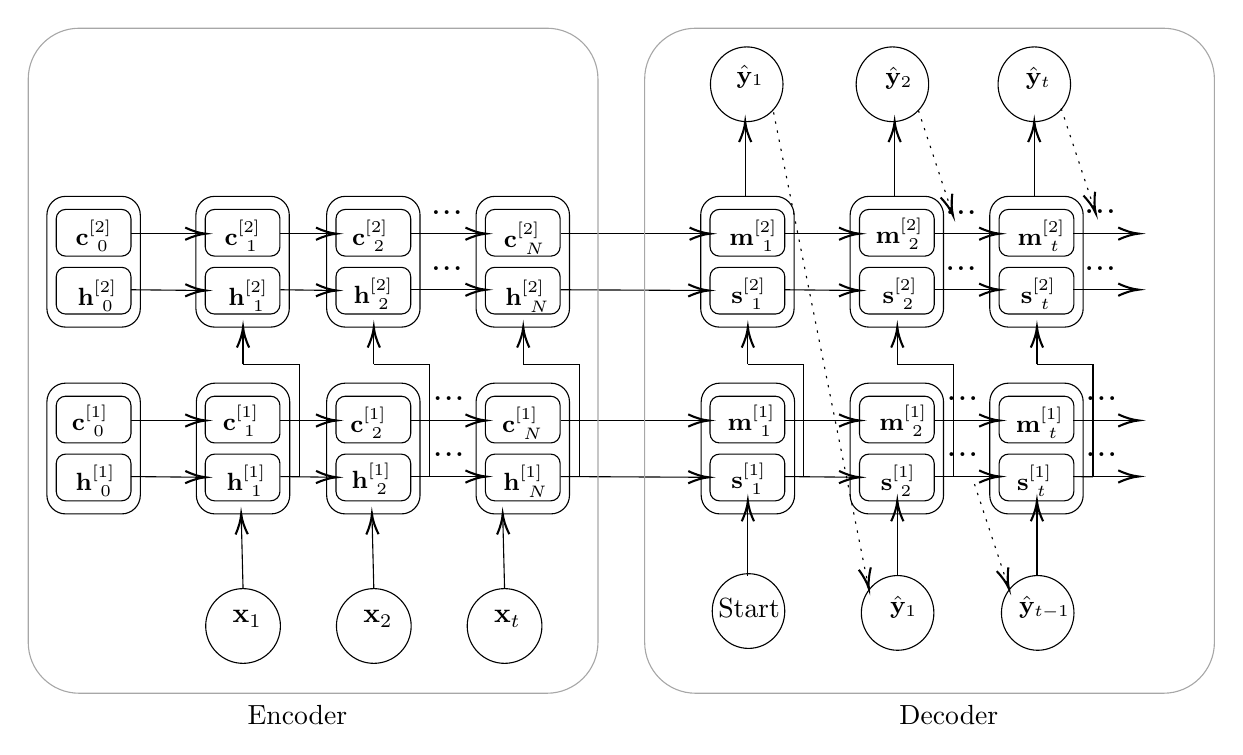
\begin{tikzpicture}[x=0.75pt,y=0.75pt,yscale=-0.9,xscale=0.9]
      %Rounded Rect [id:dp4167080735457187] 
      \draw   (95,210) .. controls (95,204.48) and (99.48,200) .. (105,200) -- (135,200) .. controls (140.52,200) and (145,204.48) .. (145,210) -- (145,260) .. controls (145,265.52) and (140.52,270) .. (135,270) -- (105,270) .. controls (99.48,270) and (95,265.52) .. (95,260) -- cycle ;
      %Rounded Rect [id:dp9346144842253596] 
      \draw   (99.75,212) .. controls (99.75,209.24) and (101.99,207) .. (104.75,207) -- (134.75,207) .. controls (137.51,207) and (139.75,209.24) .. (139.75,212) -- (139.75,227) .. controls (139.75,229.76) and (137.51,232) .. (134.75,232) -- (104.75,232) .. controls (101.99,232) and (99.75,229.76) .. (99.75,227) -- cycle ;
      %Rounded Rect [id:dp6875835908190091] 
      \draw   (99.75,243) .. controls (99.75,240.24) and (101.99,238) .. (104.75,238) -- (134.75,238) .. controls (137.51,238) and (139.75,240.24) .. (139.75,243) -- (139.75,258) .. controls (139.75,260.76) and (137.51,263) .. (134.75,263) -- (104.75,263) .. controls (101.99,263) and (99.75,260.76) .. (99.75,258) -- cycle ;
      %Shape: Ellipse [id:dp3055121979882416] 
      \draw   (100,330) .. controls (100,318.95) and (108.95,310) .. (120,310) .. controls (131.05,310) and (140,318.95) .. (140,330) .. controls (140,341.05) and (131.05,350) .. (120,350) .. controls (108.95,350) and (100,341.05) .. (100,330) -- cycle ;
      %Straight Lines [id:da9025855181913687] 
      \draw [color={rgb, 255:red, 0; green, 0; blue, 0 }  ,draw opacity=1 ]   (120,310) -- (119.05,272) ;
      \draw [shift={(119,270)}, rotate = 88.57] [color={rgb, 255:red, 0; green, 0; blue, 0 }  ,draw opacity=1 ][line width=0.75]    (10.93,-3.29) .. controls (6.95,-1.4) and (3.31,-0.3) .. (0,0) .. controls (3.31,0.3) and (6.95,1.4) .. (10.93,3.29)   ;
      %Rounded Rect [id:dp07089969288787579] 
      \draw   (15,210) .. controls (15,204.48) and (19.48,200) .. (25,200) -- (55,200) .. controls (60.52,200) and (65,204.48) .. (65,210) -- (65,260) .. controls (65,265.52) and (60.52,270) .. (55,270) -- (25,270) .. controls (19.48,270) and (15,265.52) .. (15,260) -- cycle ;
      %Rounded Rect [id:dp45824486035838286] 
      \draw   (20,212) .. controls (20,209.24) and (22.24,207) .. (25,207) -- (55,207) .. controls (57.76,207) and (60,209.24) .. (60,212) -- (60,227) .. controls (60,229.76) and (57.76,232) .. (55,232) -- (25,232) .. controls (22.24,232) and (20,229.76) .. (20,227) -- cycle ;
      %Rounded Rect [id:dp48210026138109097] 
      \draw   (20,243) .. controls (20,240.24) and (22.24,238) .. (25,238) -- (55,238) .. controls (57.76,238) and (60,240.24) .. (60,243) -- (60,258) .. controls (60,260.76) and (57.76,263) .. (55,263) -- (25,263) .. controls (22.24,263) and (20,260.76) .. (20,258) -- cycle ;
      %Straight Lines [id:da851716021162116] 
      \draw [color={rgb, 255:red, 0; green, 0; blue, 0 }  ,draw opacity=1 ]   (60,220) -- (98,220) ;
      \draw [shift={(100,220)}, rotate = 180] [color={rgb, 255:red, 0; green, 0; blue, 0 }  ,draw opacity=1 ][line width=0.75]    (10.93,-3.29) .. controls (6.95,-1.4) and (3.31,-0.3) .. (0,0) .. controls (3.31,0.3) and (6.95,1.4) .. (10.93,3.29)   ;
      %Straight Lines [id:da23842568528519448] 
      \draw [color={rgb, 255:red, 0; green, 0; blue, 0 }  ,draw opacity=1 ]   (60,250) -- (98,250.38) ;
      \draw [shift={(100,250.4)}, rotate = 180.57] [color={rgb, 255:red, 0; green, 0; blue, 0 }  ,draw opacity=1 ][line width=0.75]    (10.93,-3.29) .. controls (6.95,-1.4) and (3.31,-0.3) .. (0,0) .. controls (3.31,0.3) and (6.95,1.4) .. (10.93,3.29)   ;
      %Rounded Rect [id:dp04560159737503078] 
      \draw   (164.75,210) .. controls (164.75,204.48) and (169.23,200) .. (174.75,200) -- (204.75,200) .. controls (210.27,200) and (214.75,204.48) .. (214.75,210) -- (214.75,260) .. controls (214.75,265.52) and (210.27,270) .. (204.75,270) -- (174.75,270) .. controls (169.23,270) and (164.75,265.52) .. (164.75,260) -- cycle ;
      %Rounded Rect [id:dp08530606490144477] 
      \draw   (169.75,212) .. controls (169.75,209.24) and (171.99,207) .. (174.75,207) -- (204.75,207) .. controls (207.51,207) and (209.75,209.24) .. (209.75,212) -- (209.75,227) .. controls (209.75,229.76) and (207.51,232) .. (204.75,232) -- (174.75,232) .. controls (171.99,232) and (169.75,229.76) .. (169.75,227) -- cycle ;
      %Rounded Rect [id:dp7886901905831325] 
      \draw   (169.75,243) .. controls (169.75,240.24) and (171.99,238) .. (174.75,238) -- (204.75,238) .. controls (207.51,238) and (209.75,240.24) .. (209.75,243) -- (209.75,258) .. controls (209.75,260.76) and (207.51,263) .. (204.75,263) -- (174.75,263) .. controls (171.99,263) and (169.75,260.76) .. (169.75,258) -- cycle ;
      %Straight Lines [id:da7287683964859257] 
      \draw [color={rgb, 255:red, 0; green, 0; blue, 0 }  ,draw opacity=1 ]   (190,310) -- (189.05,272) ;
      \draw [shift={(189,270)}, rotate = 88.57] [color={rgb, 255:red, 0; green, 0; blue, 0 }  ,draw opacity=1 ][line width=0.75]    (10.93,-3.29) .. controls (6.95,-1.4) and (3.31,-0.3) .. (0,0) .. controls (3.31,0.3) and (6.95,1.4) .. (10.93,3.29)   ;
      %Straight Lines [id:da6715664171215201] 
      \draw [color={rgb, 255:red, 0; green, 0; blue, 0 }  ,draw opacity=1 ]   (140,220) -- (168,220) ;
      \draw [shift={(170,220)}, rotate = 180] [color={rgb, 255:red, 0; green, 0; blue, 0 }  ,draw opacity=1 ][line width=0.75]    (10.93,-3.29) .. controls (6.95,-1.4) and (3.31,-0.3) .. (0,0) .. controls (3.31,0.3) and (6.95,1.4) .. (10.93,3.29)   ;
      %Straight Lines [id:da6599244085959135] 
      \draw [color={rgb, 255:red, 0; green, 0; blue, 0 }  ,draw opacity=1 ]   (140,250) -- (168,250.37) ;
      \draw [shift={(170,250.4)}, rotate = 180.76] [color={rgb, 255:red, 0; green, 0; blue, 0 }  ,draw opacity=1 ][line width=0.75]    (10.93,-3.29) .. controls (6.95,-1.4) and (3.31,-0.3) .. (0,0) .. controls (3.31,0.3) and (6.95,1.4) .. (10.93,3.29)   ;
      %Rounded Rect [id:dp8902637813941603] 
      \draw   (244.75,210) .. controls (244.75,204.48) and (249.23,200) .. (254.75,200) -- (284.75,200) .. controls (290.27,200) and (294.75,204.48) .. (294.75,210) -- (294.75,260) .. controls (294.75,265.52) and (290.27,270) .. (284.75,270) -- (254.75,270) .. controls (249.23,270) and (244.75,265.52) .. (244.75,260) -- cycle ;
      %Rounded Rect [id:dp6625189643863216] 
      \draw   (249.75,212) .. controls (249.75,209.24) and (251.99,207) .. (254.75,207) -- (284.75,207) .. controls (287.51,207) and (289.75,209.24) .. (289.75,212) -- (289.75,227) .. controls (289.75,229.76) and (287.51,232) .. (284.75,232) -- (254.75,232) .. controls (251.99,232) and (249.75,229.76) .. (249.75,227) -- cycle ;
      %Rounded Rect [id:dp7778174343651048] 
      \draw   (249.75,243) .. controls (249.75,240.24) and (251.99,238) .. (254.75,238) -- (284.75,238) .. controls (287.51,238) and (289.75,240.24) .. (289.75,243) -- (289.75,258) .. controls (289.75,260.76) and (287.51,263) .. (284.75,263) -- (254.75,263) .. controls (251.99,263) and (249.75,260.76) .. (249.75,258) -- cycle ;
      %Straight Lines [id:da39906144546159594] 
      \draw [color={rgb, 255:red, 0; green, 0; blue, 0 }  ,draw opacity=1 ]   (260,310) -- (259.05,272) ;
      \draw [shift={(259,270)}, rotate = 88.57] [color={rgb, 255:red, 0; green, 0; blue, 0 }  ,draw opacity=1 ][line width=0.75]    (10.93,-3.29) .. controls (6.95,-1.4) and (3.31,-0.3) .. (0,0) .. controls (3.31,0.3) and (6.95,1.4) .. (10.93,3.29)   ;
      %Straight Lines [id:da7734816554973012] 
      \draw [color={rgb, 255:red, 0; green, 0; blue, 0 }  ,draw opacity=1 ]   (210,220) -- (248,220) ;
      \draw [shift={(250,220)}, rotate = 180] [color={rgb, 255:red, 0; green, 0; blue, 0 }  ,draw opacity=1 ][line width=0.75]    (10.93,-3.29) .. controls (6.95,-1.4) and (3.31,-0.3) .. (0,0) .. controls (3.31,0.3) and (6.95,1.4) .. (10.93,3.29)   ;
      %Straight Lines [id:da6212410028746724] 
      \draw [color={rgb, 255:red, 0; green, 0; blue, 0 }  ,draw opacity=1 ]   (210,250) -- (248,250) ;
      \draw [shift={(250,250)}, rotate = 180] [color={rgb, 255:red, 0; green, 0; blue, 0 }  ,draw opacity=1 ][line width=0.75]    (10.93,-3.29) .. controls (6.95,-1.4) and (3.31,-0.3) .. (0,0) .. controls (3.31,0.3) and (6.95,1.4) .. (10.93,3.29)   ;
      %Straight Lines [id:da6170150958930491] 
      \draw [color={rgb, 255:red, 0; green, 0; blue, 0 }  ,draw opacity=1 ]   (290,220) -- (367.25,220) ;
      \draw [shift={(369.25,220)}, rotate = 180] [color={rgb, 255:red, 0; green, 0; blue, 0 }  ,draw opacity=1 ][line width=0.75]    (10.93,-3.29) .. controls (6.95,-1.4) and (3.31,-0.3) .. (0,0) .. controls (3.31,0.3) and (6.95,1.4) .. (10.93,3.29)   ;
      %Straight Lines [id:da17036070366491862] 
      \draw [color={rgb, 255:red, 0; green, 0; blue, 0 }  ,draw opacity=1 ]   (290,250) -- (367.25,250.39) ;
      \draw [shift={(369.25,250.4)}, rotate = 180.29] [color={rgb, 255:red, 0; green, 0; blue, 0 }  ,draw opacity=1 ][line width=0.75]    (10.93,-3.29) .. controls (6.95,-1.4) and (3.31,-0.3) .. (0,0) .. controls (3.31,0.3) and (6.95,1.4) .. (10.93,3.29)   ;
      %Shape: Ellipse [id:dp921814008419761] 
      \draw   (170,330) .. controls (170,318.95) and (178.95,310) .. (190,310) .. controls (201.05,310) and (210,318.95) .. (210,330) .. controls (210,341.05) and (201.05,350) .. (190,350) .. controls (178.95,350) and (170,341.05) .. (170,330) -- cycle ;
      %Shape: Ellipse [id:dp5154518203708305] 
      \draw   (240,330) .. controls (240,318.95) and (248.95,310) .. (260,310) .. controls (271.05,310) and (280,318.95) .. (280,330) .. controls (280,341.05) and (271.05,350) .. (260,350) .. controls (248.95,350) and (240,341.05) .. (240,330) -- cycle ;
      %Rounded Rect [id:dp03092854464646244] 
      \draw   (94.75,110) .. controls (94.75,104.48) and (99.23,100) .. (104.75,100) -- (134.75,100) .. controls (140.27,100) and (144.75,104.48) .. (144.75,110) -- (144.75,160) .. controls (144.75,165.52) and (140.27,170) .. (134.75,170) -- (104.75,170) .. controls (99.23,170) and (94.75,165.52) .. (94.75,160) -- cycle ;
      %Rounded Rect [id:dp816550890492074] 
      \draw   (99.75,112) .. controls (99.75,109.24) and (101.99,107) .. (104.75,107) -- (134.75,107) .. controls (137.51,107) and (139.75,109.24) .. (139.75,112) -- (139.75,127) .. controls (139.75,129.76) and (137.51,132) .. (134.75,132) -- (104.75,132) .. controls (101.99,132) and (99.75,129.76) .. (99.75,127) -- cycle ;
      %Rounded Rect [id:dp9500665840831706] 
      \draw   (99.75,143) .. controls (99.75,140.24) and (101.99,138) .. (104.75,138) -- (134.75,138) .. controls (137.51,138) and (139.75,140.24) .. (139.75,143) -- (139.75,158) .. controls (139.75,160.76) and (137.51,163) .. (134.75,163) -- (104.75,163) .. controls (101.99,163) and (99.75,160.76) .. (99.75,158) -- cycle ;
      %Rounded Rect [id:dp3141320023119989] 
      \draw   (15,110) .. controls (15,104.48) and (19.48,100) .. (25,100) -- (55,100) .. controls (60.52,100) and (65,104.48) .. (65,110) -- (65,160) .. controls (65,165.52) and (60.52,170) .. (55,170) -- (25,170) .. controls (19.48,170) and (15,165.52) .. (15,160) -- cycle ;
      %Rounded Rect [id:dp06286358415974092] 
      \draw   (20,112) .. controls (20,109.24) and (22.24,107) .. (25,107) -- (55,107) .. controls (57.76,107) and (60,109.24) .. (60,112) -- (60,127) .. controls (60,129.76) and (57.76,132) .. (55,132) -- (25,132) .. controls (22.24,132) and (20,129.76) .. (20,127) -- cycle ;
      %Rounded Rect [id:dp09801093927348647] 
      \draw   (20,143) .. controls (20,140.24) and (22.24,138) .. (25,138) -- (55,138) .. controls (57.76,138) and (60,140.24) .. (60,143) -- (60,158) .. controls (60,160.76) and (57.76,163) .. (55,163) -- (25,163) .. controls (22.24,163) and (20,160.76) .. (20,158) -- cycle ;
      %Straight Lines [id:da026094801576276083] 
      \draw [color={rgb, 255:red, 0; green, 0; blue, 0 }  ,draw opacity=1 ]   (60,120) -- (98,120) ;
      \draw [shift={(100,120)}, rotate = 180] [color={rgb, 255:red, 0; green, 0; blue, 0 }  ,draw opacity=1 ][line width=0.75]    (10.93,-3.29) .. controls (6.95,-1.4) and (3.31,-0.3) .. (0,0) .. controls (3.31,0.3) and (6.95,1.4) .. (10.93,3.29)   ;
      %Straight Lines [id:da7209735695081336] 
      \draw [color={rgb, 255:red, 0; green, 0; blue, 0 }  ,draw opacity=1 ]   (60,150) -- (98,150.38) ;
      \draw [shift={(100,150.4)}, rotate = 180.57] [color={rgb, 255:red, 0; green, 0; blue, 0 }  ,draw opacity=1 ][line width=0.75]    (10.93,-3.29) .. controls (6.95,-1.4) and (3.31,-0.3) .. (0,0) .. controls (3.31,0.3) and (6.95,1.4) .. (10.93,3.29)   ;
      %Rounded Rect [id:dp9922570289260113] 
      \draw   (164.75,110) .. controls (164.75,104.48) and (169.23,100) .. (174.75,100) -- (204.75,100) .. controls (210.27,100) and (214.75,104.48) .. (214.75,110) -- (214.75,160) .. controls (214.75,165.52) and (210.27,170) .. (204.75,170) -- (174.75,170) .. controls (169.23,170) and (164.75,165.52) .. (164.75,160) -- cycle ;
      %Rounded Rect [id:dp9753501113257226] 
      \draw   (169.75,112) .. controls (169.75,109.24) and (171.99,107) .. (174.75,107) -- (204.75,107) .. controls (207.51,107) and (209.75,109.24) .. (209.75,112) -- (209.75,127) .. controls (209.75,129.76) and (207.51,132) .. (204.75,132) -- (174.75,132) .. controls (171.99,132) and (169.75,129.76) .. (169.75,127) -- cycle ;
      %Rounded Rect [id:dp39752964789027234] 
      \draw   (169.75,143) .. controls (169.75,140.24) and (171.99,138) .. (174.75,138) -- (204.75,138) .. controls (207.51,138) and (209.75,140.24) .. (209.75,143) -- (209.75,158) .. controls (209.75,160.76) and (207.51,163) .. (204.75,163) -- (174.75,163) .. controls (171.99,163) and (169.75,160.76) .. (169.75,158) -- cycle ;
      %Straight Lines [id:da7201454739572428] 
      \draw [color={rgb, 255:red, 0; green, 0; blue, 0 }  ,draw opacity=1 ]   (140,120) -- (168,120) ;
      \draw [shift={(170,120)}, rotate = 180] [color={rgb, 255:red, 0; green, 0; blue, 0 }  ,draw opacity=1 ][line width=0.75]    (10.93,-3.29) .. controls (6.95,-1.4) and (3.31,-0.3) .. (0,0) .. controls (3.31,0.3) and (6.95,1.4) .. (10.93,3.29)   ;
      %Straight Lines [id:da714248693226855] 
      \draw [color={rgb, 255:red, 0; green, 0; blue, 0 }  ,draw opacity=1 ]   (140,150) -- (168,150.37) ;
      \draw [shift={(170,150.4)}, rotate = 180.76] [color={rgb, 255:red, 0; green, 0; blue, 0 }  ,draw opacity=1 ][line width=0.75]    (10.93,-3.29) .. controls (6.95,-1.4) and (3.31,-0.3) .. (0,0) .. controls (3.31,0.3) and (6.95,1.4) .. (10.93,3.29)   ;
      %Rounded Rect [id:dp9710143758385796] 
      \draw   (244.75,110) .. controls (244.75,104.48) and (249.23,100) .. (254.75,100) -- (284.75,100) .. controls (290.27,100) and (294.75,104.48) .. (294.75,110) -- (294.75,160) .. controls (294.75,165.52) and (290.27,170) .. (284.75,170) -- (254.75,170) .. controls (249.23,170) and (244.75,165.52) .. (244.75,160) -- cycle ;
      %Rounded Rect [id:dp6076792282358365] 
      \draw   (249.75,112) .. controls (249.75,109.24) and (251.99,107) .. (254.75,107) -- (284.75,107) .. controls (287.51,107) and (289.75,109.24) .. (289.75,112) -- (289.75,127) .. controls (289.75,129.76) and (287.51,132) .. (284.75,132) -- (254.75,132) .. controls (251.99,132) and (249.75,129.76) .. (249.75,127) -- cycle ;
      %Rounded Rect [id:dp8301870485368747] 
      \draw   (249.75,143) .. controls (249.75,140.24) and (251.99,138) .. (254.75,138) -- (284.75,138) .. controls (287.51,138) and (289.75,140.24) .. (289.75,143) -- (289.75,158) .. controls (289.75,160.76) and (287.51,163) .. (284.75,163) -- (254.75,163) .. controls (251.99,163) and (249.75,160.76) .. (249.75,158) -- cycle ;
      %Straight Lines [id:da18021147009414817] 
      \draw [color={rgb, 255:red, 0; green, 0; blue, 0 }  ,draw opacity=1 ]   (210,120) -- (248,120) ;
      \draw [shift={(250,120)}, rotate = 180] [color={rgb, 255:red, 0; green, 0; blue, 0 }  ,draw opacity=1 ][line width=0.75]    (10.93,-3.29) .. controls (6.95,-1.4) and (3.31,-0.3) .. (0,0) .. controls (3.31,0.3) and (6.95,1.4) .. (10.93,3.29)   ;
      %Straight Lines [id:da9792801142158605] 
      \draw [color={rgb, 255:red, 0; green, 0; blue, 0 }  ,draw opacity=1 ]   (210,150) -- (248,150) ;
      \draw [shift={(250,150)}, rotate = 180] [color={rgb, 255:red, 0; green, 0; blue, 0 }  ,draw opacity=1 ][line width=0.75]    (10.93,-3.29) .. controls (6.95,-1.4) and (3.31,-0.3) .. (0,0) .. controls (3.31,0.3) and (6.95,1.4) .. (10.93,3.29)   ;
      %Straight Lines [id:da09217962764014365] 
      \draw [color={rgb, 255:red, 0; green, 0; blue, 0 }  ,draw opacity=1 ]   (290,120) -- (368,120) ;
      \draw [shift={(370,120)}, rotate = 180] [color={rgb, 255:red, 0; green, 0; blue, 0 }  ,draw opacity=1 ][line width=0.75]    (10.93,-3.29) .. controls (6.95,-1.4) and (3.31,-0.3) .. (0,0) .. controls (3.31,0.3) and (6.95,1.4) .. (10.93,3.29)   ;
      %Straight Lines [id:da07024764866360234] 
      \draw [color={rgb, 255:red, 0; green, 0; blue, 0 }  ,draw opacity=1 ]   (290,150) -- (367.25,150.39) ;
      \draw [shift={(369.25,150.4)}, rotate = 180.29] [color={rgb, 255:red, 0; green, 0; blue, 0 }  ,draw opacity=1 ][line width=0.75]    (10.93,-3.29) .. controls (6.95,-1.4) and (3.31,-0.3) .. (0,0) .. controls (3.31,0.3) and (6.95,1.4) .. (10.93,3.29)   ;
      %Straight Lines [id:da8792682771837725] 
      \draw    (150,250.2) -- (150,190) ;
      %Straight Lines [id:da2634240032707502] 
      \draw    (120,190) -- (150,190) ;
      %Straight Lines [id:da12484928851738863] 
      \draw    (120,190) -- (120,172) ;
      \draw [shift={(120,170)}, rotate = 90] [color={rgb, 255:red, 0; green, 0; blue, 0 }  ][line width=0.75]    (10.93,-3.29) .. controls (6.95,-1.4) and (3.31,-0.3) .. (0,0) .. controls (3.31,0.3) and (6.95,1.4) .. (10.93,3.29)   ;
      %Straight Lines [id:da5759992375631084] 
      \draw    (220,250.2) -- (220,190) ;
      %Straight Lines [id:da5103327101821591] 
      \draw    (190,190) -- (220,190) ;
      %Straight Lines [id:da7509876273419771] 
      \draw    (190,190) -- (190,172) ;
      \draw [shift={(190,170)}, rotate = 90] [color={rgb, 255:red, 0; green, 0; blue, 0 }  ][line width=0.75]    (10.93,-3.29) .. controls (6.95,-1.4) and (3.31,-0.3) .. (0,0) .. controls (3.31,0.3) and (6.95,1.4) .. (10.93,3.29)   ;
      %Straight Lines [id:da15793149664296036] 
      \draw    (270,190) -- (300,190) ;
      %Straight Lines [id:da4796232669148728] 
      \draw    (270,190) -- (270,172) ;
      \draw [shift={(270,170)}, rotate = 90] [color={rgb, 255:red, 0; green, 0; blue, 0 }  ][line width=0.75]    (10.93,-3.29) .. controls (6.95,-1.4) and (3.31,-0.3) .. (0,0) .. controls (3.31,0.3) and (6.95,1.4) .. (10.93,3.29)   ;
      %Straight Lines [id:da700877547716785] 
      \draw    (300,250.2) -- (300,190) ;
      %Rounded Rect [id:dp8674888716756768] 
      \draw   (365.25,210) .. controls (365.25,204.48) and (369.73,200) .. (375.25,200) -- (405.25,200) .. controls (410.77,200) and (415.25,204.48) .. (415.25,210) -- (415.25,260) .. controls (415.25,265.52) and (410.77,270) .. (405.25,270) -- (375.25,270) .. controls (369.73,270) and (365.25,265.52) .. (365.25,260) -- cycle ;
      %Rounded Rect [id:dp5489391539785766] 
      \draw   (370,212) .. controls (370,209.24) and (372.24,207) .. (375,207) -- (405,207) .. controls (407.76,207) and (410,209.24) .. (410,212) -- (410,227) .. controls (410,229.76) and (407.76,232) .. (405,232) -- (375,232) .. controls (372.24,232) and (370,229.76) .. (370,227) -- cycle ;
      %Rounded Rect [id:dp5963099944409156] 
      \draw   (370,243) .. controls (370,240.24) and (372.24,238) .. (375,238) -- (405,238) .. controls (407.76,238) and (410,240.24) .. (410,243) -- (410,258) .. controls (410,260.76) and (407.76,263) .. (405,263) -- (375,263) .. controls (372.24,263) and (370,260.76) .. (370,258) -- cycle ;
      %Straight Lines [id:da911979939972424] 
      \draw [color={rgb, 255:red, 0; green, 0; blue, 0 }  ,draw opacity=1 ]   (388.82,100) -- (388.82,66) -- (388.82,62) ;
      \draw [shift={(388.82,60)}, rotate = 90] [color={rgb, 255:red, 0; green, 0; blue, 0 }  ,draw opacity=1 ][line width=0.75]    (10.93,-3.29) .. controls (6.95,-1.4) and (3.31,-0.3) .. (0,0) .. controls (3.31,0.3) and (6.95,1.4) .. (10.93,3.29)   ;
      %Rounded Rect [id:dp7221083753374034] 
      \draw   (445,210) .. controls (445,204.48) and (449.48,200) .. (455,200) -- (485,200) .. controls (490.52,200) and (495,204.48) .. (495,210) -- (495,260) .. controls (495,265.52) and (490.52,270) .. (485,270) -- (455,270) .. controls (449.48,270) and (445,265.52) .. (445,260) -- cycle ;
      %Rounded Rect [id:dp36860252170123875] 
      \draw   (450,212) .. controls (450,209.24) and (452.24,207) .. (455,207) -- (485,207) .. controls (487.76,207) and (490,209.24) .. (490,212) -- (490,227) .. controls (490,229.76) and (487.76,232) .. (485,232) -- (455,232) .. controls (452.24,232) and (450,229.76) .. (450,227) -- cycle ;
      %Rounded Rect [id:dp6114065023247515] 
      \draw   (450,243) .. controls (450,240.24) and (452.24,238) .. (455,238) -- (485,238) .. controls (487.76,238) and (490,240.24) .. (490,243) -- (490,258) .. controls (490,260.76) and (487.76,263) .. (485,263) -- (455,263) .. controls (452.24,263) and (450,260.76) .. (450,258) -- cycle ;
      %Straight Lines [id:da6816491393136734] 
      \draw [color={rgb, 255:red, 0; green, 0; blue, 0 }  ,draw opacity=1 ]   (468.82,100) -- (468.82,66) -- (468.82,62) ;
      \draw [shift={(468.82,60)}, rotate = 90] [color={rgb, 255:red, 0; green, 0; blue, 0 }  ,draw opacity=1 ][line width=0.75]    (10.93,-3.29) .. controls (6.95,-1.4) and (3.31,-0.3) .. (0,0) .. controls (3.31,0.3) and (6.95,1.4) .. (10.93,3.29)   ;
      %Rounded Rect [id:dp509214694654305] 
      \draw   (519.75,210) .. controls (519.75,204.48) and (524.23,200) .. (529.75,200) -- (559.75,200) .. controls (565.27,200) and (569.75,204.48) .. (569.75,210) -- (569.75,260) .. controls (569.75,265.52) and (565.27,270) .. (559.75,270) -- (529.75,270) .. controls (524.23,270) and (519.75,265.52) .. (519.75,260) -- cycle ;
      %Rounded Rect [id:dp41118491999009565] 
      \draw   (524.75,212) .. controls (524.75,209.24) and (526.99,207) .. (529.75,207) -- (559.75,207) .. controls (562.51,207) and (564.75,209.24) .. (564.75,212) -- (564.75,227) .. controls (564.75,229.76) and (562.51,232) .. (559.75,232) -- (529.75,232) .. controls (526.99,232) and (524.75,229.76) .. (524.75,227) -- cycle ;
      %Rounded Rect [id:dp04750143326593914] 
      \draw   (524.75,243) .. controls (524.75,240.24) and (526.99,238) .. (529.75,238) -- (559.75,238) .. controls (562.51,238) and (564.75,240.24) .. (564.75,243) -- (564.75,258) .. controls (564.75,260.76) and (562.51,263) .. (559.75,263) -- (529.75,263) .. controls (526.99,263) and (524.75,260.76) .. (524.75,258) -- cycle ;
      %Straight Lines [id:da8817473076349263] 
      \draw [color={rgb, 255:red, 0; green, 0; blue, 0 }  ,draw opacity=1 ]   (543.57,100) -- (543.57,66) -- (543.57,62) ;
      \draw [shift={(543.57,60)}, rotate = 90] [color={rgb, 255:red, 0; green, 0; blue, 0 }  ,draw opacity=1 ][line width=0.75]    (10.93,-3.29) .. controls (6.95,-1.4) and (3.31,-0.3) .. (0,0) .. controls (3.31,0.3) and (6.95,1.4) .. (10.93,3.29)   ;
      %Straight Lines [id:da27286644665918924] 
      \draw [color={rgb, 255:red, 0; green, 0; blue, 0 }  ,draw opacity=1 ]   (410,220) -- (448,220) ;
      \draw [shift={(450,220)}, rotate = 180] [color={rgb, 255:red, 0; green, 0; blue, 0 }  ,draw opacity=1 ][line width=0.75]    (10.93,-3.29) .. controls (6.95,-1.4) and (3.31,-0.3) .. (0,0) .. controls (3.31,0.3) and (6.95,1.4) .. (10.93,3.29)   ;
      %Straight Lines [id:da9479965742141365] 
      \draw [color={rgb, 255:red, 0; green, 0; blue, 0 }  ,draw opacity=1 ]   (410,250) -- (448,250.38) ;
      \draw [shift={(450,250.4)}, rotate = 180.57] [color={rgb, 255:red, 0; green, 0; blue, 0 }  ,draw opacity=1 ][line width=0.75]    (10.93,-3.29) .. controls (6.95,-1.4) and (3.31,-0.3) .. (0,0) .. controls (3.31,0.3) and (6.95,1.4) .. (10.93,3.29)   ;
      %Rounded Rect [id:dp19540509121782024] 
      \draw   (365,110) .. controls (365,104.48) and (369.48,100) .. (375,100) -- (405,100) .. controls (410.52,100) and (415,104.48) .. (415,110) -- (415,160) .. controls (415,165.52) and (410.52,170) .. (405,170) -- (375,170) .. controls (369.48,170) and (365,165.52) .. (365,160) -- cycle ;
      %Rounded Rect [id:dp2762867928089998] 
      \draw   (370,112) .. controls (370,109.24) and (372.24,107) .. (375,107) -- (405,107) .. controls (407.76,107) and (410,109.24) .. (410,112) -- (410,127) .. controls (410,129.76) and (407.76,132) .. (405,132) -- (375,132) .. controls (372.24,132) and (370,129.76) .. (370,127) -- cycle ;
      %Rounded Rect [id:dp9587780841664757] 
      \draw   (370,143) .. controls (370,140.24) and (372.24,138) .. (375,138) -- (405,138) .. controls (407.76,138) and (410,140.24) .. (410,143) -- (410,158) .. controls (410,160.76) and (407.76,163) .. (405,163) -- (375,163) .. controls (372.24,163) and (370,160.76) .. (370,158) -- cycle ;
      %Rounded Rect [id:dp5296850448101615] 
      \draw   (445,110) .. controls (445,104.48) and (449.48,100) .. (455,100) -- (485,100) .. controls (490.52,100) and (495,104.48) .. (495,110) -- (495,160) .. controls (495,165.52) and (490.52,170) .. (485,170) -- (455,170) .. controls (449.48,170) and (445,165.52) .. (445,160) -- cycle ;
      %Rounded Rect [id:dp7925349138834241] 
      \draw   (450,112) .. controls (450,109.24) and (452.24,107) .. (455,107) -- (485,107) .. controls (487.76,107) and (490,109.24) .. (490,112) -- (490,127) .. controls (490,129.76) and (487.76,132) .. (485,132) -- (455,132) .. controls (452.24,132) and (450,129.76) .. (450,127) -- cycle ;
      %Rounded Rect [id:dp10913626409203814] 
      \draw   (450,143) .. controls (450,140.24) and (452.24,138) .. (455,138) -- (485,138) .. controls (487.76,138) and (490,140.24) .. (490,143) -- (490,158) .. controls (490,160.76) and (487.76,163) .. (485,163) -- (455,163) .. controls (452.24,163) and (450,160.76) .. (450,158) -- cycle ;
      %Rounded Rect [id:dp23474579373402982] 
      \draw   (519.75,110) .. controls (519.75,104.48) and (524.23,100) .. (529.75,100) -- (559.75,100) .. controls (565.27,100) and (569.75,104.48) .. (569.75,110) -- (569.75,160) .. controls (569.75,165.52) and (565.27,170) .. (559.75,170) -- (529.75,170) .. controls (524.23,170) and (519.75,165.52) .. (519.75,160) -- cycle ;
      %Rounded Rect [id:dp08285224899170052] 
      \draw   (524.75,112) .. controls (524.75,109.24) and (526.99,107) .. (529.75,107) -- (559.75,107) .. controls (562.51,107) and (564.75,109.24) .. (564.75,112) -- (564.75,127) .. controls (564.75,129.76) and (562.51,132) .. (559.75,132) -- (529.75,132) .. controls (526.99,132) and (524.75,129.76) .. (524.75,127) -- cycle ;
      %Rounded Rect [id:dp09356096334165964] 
      \draw   (524.75,143) .. controls (524.75,140.24) and (526.99,138) .. (529.75,138) -- (559.75,138) .. controls (562.51,138) and (564.75,140.24) .. (564.75,143) -- (564.75,158) .. controls (564.75,160.76) and (562.51,163) .. (559.75,163) -- (529.75,163) .. controls (526.99,163) and (524.75,160.76) .. (524.75,158) -- cycle ;
      %Straight Lines [id:da2630583353195102] 
      \draw [color={rgb, 255:red, 0; green, 0; blue, 0 }  ,draw opacity=1 ]   (410,120) -- (448,120) ;
      \draw [shift={(450,120)}, rotate = 180] [color={rgb, 255:red, 0; green, 0; blue, 0 }  ,draw opacity=1 ][line width=0.75]    (10.93,-3.29) .. controls (6.95,-1.4) and (3.31,-0.3) .. (0,0) .. controls (3.31,0.3) and (6.95,1.4) .. (10.93,3.29)   ;
      %Straight Lines [id:da9003673432635384] 
      \draw [color={rgb, 255:red, 0; green, 0; blue, 0 }  ,draw opacity=1 ]   (410,150) -- (448,150.38) ;
      \draw [shift={(450,150.4)}, rotate = 180.57] [color={rgb, 255:red, 0; green, 0; blue, 0 }  ,draw opacity=1 ][line width=0.75]    (10.93,-3.29) .. controls (6.95,-1.4) and (3.31,-0.3) .. (0,0) .. controls (3.31,0.3) and (6.95,1.4) .. (10.93,3.29)   ;
      %Straight Lines [id:da6304538683356946] 
      \draw    (420.25,250.2) -- (420.25,190) ;
      %Straight Lines [id:da8370681679149368] 
      \draw    (390.25,190) -- (420.25,190) ;
      %Straight Lines [id:da36413170867480615] 
      \draw    (390.25,190) -- (390.25,172) ;
      \draw [shift={(390.25,170)}, rotate = 90] [color={rgb, 255:red, 0; green, 0; blue, 0 }  ][line width=0.75]    (10.93,-3.29) .. controls (6.95,-1.4) and (3.31,-0.3) .. (0,0) .. controls (3.31,0.3) and (6.95,1.4) .. (10.93,3.29)   ;
      %Straight Lines [id:da02263779133221222] 
      \draw    (500.25,250.2) -- (500.25,190) ;
      %Straight Lines [id:da6321066586201223] 
      \draw    (470.25,190) -- (500.25,190) ;
      %Straight Lines [id:da9741545158763674] 
      \draw    (470.25,190) -- (470.25,172) ;
      \draw [shift={(470.25,170)}, rotate = 90] [color={rgb, 255:red, 0; green, 0; blue, 0 }  ][line width=0.75]    (10.93,-3.29) .. controls (6.95,-1.4) and (3.31,-0.3) .. (0,0) .. controls (3.31,0.3) and (6.95,1.4) .. (10.93,3.29)   ;
      %Straight Lines [id:da47873868152464216] 
      \draw    (575,250.2) -- (575,190) ;
      %Straight Lines [id:da6668557121227057] 
      \draw    (545,190) -- (575,190) ;
      %Straight Lines [id:da12904452588003146] 
      \draw    (545,190) -- (545,172) ;
      \draw [shift={(545,170)}, rotate = 90] [color={rgb, 255:red, 0; green, 0; blue, 0 }  ][line width=0.75]    (10.93,-3.29) .. controls (6.95,-1.4) and (3.31,-0.3) .. (0,0) .. controls (3.31,0.3) and (6.95,1.4) .. (10.93,3.29)   ;
      %Straight Lines [id:da7293210834974657] 
      \draw [color={rgb, 255:red, 0; green, 0; blue, 0 }  ,draw opacity=1 ]   (490,220) -- (523,220) ;
      \draw [shift={(525,220)}, rotate = 180] [color={rgb, 255:red, 0; green, 0; blue, 0 }  ,draw opacity=1 ][line width=0.75]    (10.93,-3.29) .. controls (6.95,-1.4) and (3.31,-0.3) .. (0,0) .. controls (3.31,0.3) and (6.95,1.4) .. (10.93,3.29)   ;
      %Straight Lines [id:da1064022544729053] 
      \draw [color={rgb, 255:red, 0; green, 0; blue, 0 }  ,draw opacity=1 ]   (490,250) -- (523,250) ;
      \draw [shift={(525,250)}, rotate = 180] [color={rgb, 255:red, 0; green, 0; blue, 0 }  ,draw opacity=1 ][line width=0.75]    (10.93,-3.29) .. controls (6.95,-1.4) and (3.31,-0.3) .. (0,0) .. controls (3.31,0.3) and (6.95,1.4) .. (10.93,3.29)   ;
      %Straight Lines [id:da07130857733309437] 
      \draw [color={rgb, 255:red, 0; green, 0; blue, 0 }  ,draw opacity=1 ]   (490,120) -- (523,120) ;
      \draw [shift={(525,120)}, rotate = 180] [color={rgb, 255:red, 0; green, 0; blue, 0 }  ,draw opacity=1 ][line width=0.75]    (10.93,-3.29) .. controls (6.95,-1.4) and (3.31,-0.3) .. (0,0) .. controls (3.31,0.3) and (6.95,1.4) .. (10.93,3.29)   ;
      %Straight Lines [id:da7312641973991214] 
      \draw [color={rgb, 255:red, 0; green, 0; blue, 0 }  ,draw opacity=1 ]   (490,150) -- (523,150) ;
      \draw [shift={(525,150)}, rotate = 180] [color={rgb, 255:red, 0; green, 0; blue, 0 }  ,draw opacity=1 ][line width=0.75]    (10.93,-3.29) .. controls (6.95,-1.4) and (3.31,-0.3) .. (0,0) .. controls (3.31,0.3) and (6.95,1.4) .. (10.93,3.29)   ;
      %Straight Lines [id:da9300102498701175] 
      \draw    (565,250) -- (575,250.2) ;
      %Rounded Rect [id:dp3317617565588511] 
      \draw  [color={rgb, 255:red, 167; green, 167; blue, 167 }  ,draw opacity=1 ] (5,37.26) .. controls (5,22.2) and (17.2,10) .. (32.26,10) -- (282.74,10) .. controls (297.8,10) and (310,22.2) .. (310,37.26) -- (310,338.74) .. controls (310,353.8) and (297.8,366) .. (282.74,366) -- (32.26,366) .. controls (17.2,366) and (5,353.8) .. (5,338.74) -- cycle ;
      %Rounded Rect [id:dp5783177244986819] 
      \draw  [color={rgb, 255:red, 167; green, 167; blue, 167 }  ,draw opacity=1 ] (335,37.26) .. controls (335,22.2) and (347.2,10) .. (362.26,10) -- (612.74,10) .. controls (627.8,10) and (640,22.2) .. (640,37.26) -- (640,338.74) .. controls (640,353.8) and (627.8,366) .. (612.74,366) -- (362.26,366) .. controls (347.2,366) and (335,353.8) .. (335,338.74) -- cycle ;
      %Shape: Ellipse [id:dp7733394302286176] 
      \draw   (448.22,40) .. controls (448.22,28.95) and (456.91,20) .. (467.63,20) .. controls (478.35,20) and (487.04,28.95) .. (487.04,40) .. controls (487.04,51.05) and (478.35,60) .. (467.63,60) .. controls (456.91,60) and (448.22,51.05) .. (448.22,40) -- cycle ;
      %Shape: Ellipse [id:dp6556072395259707] 
      \draw   (524.18,40) .. controls (524.18,28.95) and (532.87,20) .. (543.59,20) .. controls (554.31,20) and (563,28.95) .. (563,40) .. controls (563,51.05) and (554.31,60) .. (543.59,60) .. controls (532.87,60) and (524.18,51.05) .. (524.18,40) -- cycle ;
      %Shape: Ellipse [id:dp3170085190999692] 
      \draw   (370.22,40) .. controls (370.22,28.95) and (378.91,20) .. (389.64,20) .. controls (400.36,20) and (409.05,28.95) .. (409.05,40) .. controls (409.05,51.05) and (400.36,60) .. (389.64,60) .. controls (378.91,60) and (370.22,51.05) .. (370.22,40) -- cycle ;
      %Straight Lines [id:da1470169361742475] 
      \draw [color={rgb, 255:red, 0; green, 0; blue, 0 }  ,draw opacity=1 ]   (390.25,303) -- (390.25,269) -- (390.25,265) ;
      \draw [shift={(390.25,263)}, rotate = 90] [color={rgb, 255:red, 0; green, 0; blue, 0 }  ,draw opacity=1 ][line width=0.75]    (10.93,-3.29) .. controls (6.95,-1.4) and (3.31,-0.3) .. (0,0) .. controls (3.31,0.3) and (6.95,1.4) .. (10.93,3.29)   ;
      %Straight Lines [id:da41901171346149146] 
      \draw [color={rgb, 255:red, 0; green, 0; blue, 0 }  ,draw opacity=1 ]   (470.25,303) -- (470.25,269) -- (470.25,265) ;
      \draw [shift={(470.25,263)}, rotate = 90] [color={rgb, 255:red, 0; green, 0; blue, 0 }  ,draw opacity=1 ][line width=0.75]    (10.93,-3.29) .. controls (6.95,-1.4) and (3.31,-0.3) .. (0,0) .. controls (3.31,0.3) and (6.95,1.4) .. (10.93,3.29)   ;
      %Straight Lines [id:da9442497190844032] 
      \draw [color={rgb, 255:red, 0; green, 0; blue, 0 }  ,draw opacity=1 ]   (545,303) -- (545,269) -- (545,265) ;
      \draw [shift={(545,263)}, rotate = 90] [color={rgb, 255:red, 0; green, 0; blue, 0 }  ,draw opacity=1 ][line width=0.75]    (10.93,-3.29) .. controls (6.95,-1.4) and (3.31,-0.3) .. (0,0) .. controls (3.31,0.3) and (6.95,1.4) .. (10.93,3.29)   ;
      %Shape: Ellipse [id:dp26075433324765007] 
      \draw   (451,323) .. controls (451,311.95) and (459.69,303) .. (470.41,303) .. controls (481.13,303) and (489.82,311.95) .. (489.82,323) .. controls (489.82,334.05) and (481.13,343) .. (470.41,343) .. controls (459.69,343) and (451,334.05) .. (451,323) -- cycle ;
      %Shape: Ellipse [id:dp9999850289764194] 
      \draw   (526,323) .. controls (526,311.95) and (534.69,303) .. (545.41,303) .. controls (556.13,303) and (564.82,311.95) .. (564.82,323) .. controls (564.82,334.05) and (556.13,343) .. (545.41,343) .. controls (534.69,343) and (526,334.05) .. (526,323) -- cycle ;
      %Shape: Ellipse [id:dp9467729465080421] 
      \draw   (371.18,322) .. controls (371.18,310.95) and (379.87,302) .. (390.59,302) .. controls (401.31,302) and (410,310.95) .. (410,322) .. controls (410,333.05) and (401.31,342) .. (390.59,342) .. controls (379.87,342) and (371.18,333.05) .. (371.18,322) -- cycle ;
      %Straight Lines [id:da027983118369862225] 
      \draw  [dash pattern={on 0.84pt off 2.51pt}]  (404,55) -- (454.61,308.04) ;
      \draw [shift={(455,310)}, rotate = 258.69] [color={rgb, 255:red, 0; green, 0; blue, 0 }  ][line width=0.75]    (10.93,-3.29) .. controls (6.95,-1.4) and (3.31,-0.3) .. (0,0) .. controls (3.31,0.3) and (6.95,1.4) .. (10.93,3.29)   ;
      %Straight Lines [id:da421370449385543] 
      \draw  [dash pattern={on 0.84pt off 2.51pt}]  (481.55,54.04) -- (499.37,108.1) ;
      \draw [shift={(500,110)}, rotate = 251.75] [color={rgb, 255:red, 0; green, 0; blue, 0 }  ][line width=0.75]    (10.93,-3.29) .. controls (6.95,-1.4) and (3.31,-0.3) .. (0,0) .. controls (3.31,0.3) and (6.95,1.4) .. (10.93,3.29)   ;
      %Straight Lines [id:da7826555051462878] 
      \draw [color={rgb, 255:red, 0; green, 0; blue, 0 }  ,draw opacity=1 ]   (564.45,219.96) -- (597.45,219.96) ;
      \draw [shift={(599.45,219.96)}, rotate = 180] [color={rgb, 255:red, 0; green, 0; blue, 0 }  ,draw opacity=1 ][line width=0.75]    (10.93,-3.29) .. controls (6.95,-1.4) and (3.31,-0.3) .. (0,0) .. controls (3.31,0.3) and (6.95,1.4) .. (10.93,3.29)   ;
      %Straight Lines [id:da45270197344696106] 
      \draw [color={rgb, 255:red, 0; green, 0; blue, 0 }  ,draw opacity=1 ]   (564.45,249.96) -- (597.45,249.96) ;
      \draw [shift={(599.45,249.96)}, rotate = 180] [color={rgb, 255:red, 0; green, 0; blue, 0 }  ,draw opacity=1 ][line width=0.75]    (10.93,-3.29) .. controls (6.95,-1.4) and (3.31,-0.3) .. (0,0) .. controls (3.31,0.3) and (6.95,1.4) .. (10.93,3.29)   ;
      %Straight Lines [id:da6533397571061048] 
      \draw [color={rgb, 255:red, 0; green, 0; blue, 0 }  ,draw opacity=1 ]   (564.45,119.96) -- (597.45,119.96) ;
      \draw [shift={(599.45,119.96)}, rotate = 180] [color={rgb, 255:red, 0; green, 0; blue, 0 }  ,draw opacity=1 ][line width=0.75]    (10.93,-3.29) .. controls (6.95,-1.4) and (3.31,-0.3) .. (0,0) .. controls (3.31,0.3) and (6.95,1.4) .. (10.93,3.29)   ;
      %Straight Lines [id:da5060182014403987] 
      \draw [color={rgb, 255:red, 0; green, 0; blue, 0 }  ,draw opacity=1 ]   (564.45,149.96) -- (597.45,149.96) ;
      \draw [shift={(599.45,149.96)}, rotate = 180] [color={rgb, 255:red, 0; green, 0; blue, 0 }  ,draw opacity=1 ][line width=0.75]    (10.93,-3.29) .. controls (6.95,-1.4) and (3.31,-0.3) .. (0,0) .. controls (3.31,0.3) and (6.95,1.4) .. (10.93,3.29)   ;
      %Straight Lines [id:da887931619832435] 
      \draw  [dash pattern={on 0.84pt off 2.51pt}]  (511.55,254.04) -- (529.37,308.1) ;
      \draw [shift={(530,310)}, rotate = 251.75] [color={rgb, 255:red, 0; green, 0; blue, 0 }  ][line width=0.75]    (10.93,-3.29) .. controls (6.95,-1.4) and (3.31,-0.3) .. (0,0) .. controls (3.31,0.3) and (6.95,1.4) .. (10.93,3.29)   ;
      %Straight Lines [id:da904024081259367] 
      \draw  [dash pattern={on 0.84pt off 2.51pt}]  (558,53) -- (575.83,107.06) ;
      \draw [shift={(576.45,108.96)}, rotate = 251.75] [color={rgb, 255:red, 0; green, 0; blue, 0 }  ][line width=0.75]    (10.93,-3.29) .. controls (6.95,-1.4) and (3.31,-0.3) .. (0,0) .. controls (3.31,0.3) and (6.95,1.4) .. (10.93,3.29)   ;

      % Text Node
      \draw (113,320.4) node [anchor=north west][inner sep=0.75pt]  [font=\normalsize]  {$\mathbf{x}_{1}$};
      % Text Node
      \draw (220,206) node [anchor=north west][inner sep=0.75pt]  [font=\Large] [align=left] {...};
      % Text Node
      \draw (220,236) node [anchor=north west][inner sep=0.75pt]  [font=\Large] [align=left] {...};
      % Text Node
      \draw (183,320.4) node [anchor=north west][inner sep=0.75pt]  [font=\normalsize]  {$\mathbf{x}_{2}$};
      % Text Node
      \draw (253,320.4) node [anchor=north west][inner sep=0.75pt]  [font=\normalsize]  {$\mathbf{x}_{t}$};
      % Text Node
      \draw (110.75,143.4) node [anchor=north west][inner sep=0.75pt]  [font=\small]  {$\mathbf{h}_{\ 1}^{[ 2]}$};
      % Text Node
      \draw (108.75,111.4) node [anchor=north west][inner sep=0.75pt]  [font=\small]  {$\mathbf{c}_{\ 1}^{[ 2]}$};
      % Text Node
      \draw (30,143.4) node [anchor=north west][inner sep=0.75pt]  [font=\small]  {$\mathbf{h}_{\ 0}^{[ 2]}$};
      % Text Node
      \draw (29,111.4) node [anchor=north west][inner sep=0.75pt]  [font=\small]  {$\mathbf{c}_{\ 0}^{[ 2]}$};
      % Text Node
      \draw (219,106) node [anchor=north west][inner sep=0.75pt]  [font=\Large] [align=left] {...};
      % Text Node
      \draw (219,136) node [anchor=north west][inner sep=0.75pt]  [font=\Large] [align=left] {...};
      % Text Node
      \draw (177.75,142.4) node [anchor=north west][inner sep=0.75pt]  [font=\small]  {$\mathbf{h}_{\ 2}^{[ 2]}$};
      % Text Node
      \draw (177,111.4) node [anchor=north west][inner sep=0.75pt]  [font=\small]  {$\mathbf{c}_{\ 2}^{[ 2]}$};
      % Text Node
      \draw (259,143.4) node [anchor=north west][inner sep=0.75pt]  [font=\small]  {$\mathbf{h}_{\ N}^{[ 2]}$};
      % Text Node
      \draw (258.25,112.4) node [anchor=north west][inner sep=0.75pt]  [font=\small]  {$\mathbf{c}_{\ N}^{[ 2]}$};
      % Text Node
      \draw (109.75,242.4) node [anchor=north west][inner sep=0.75pt]  [font=\small]  {$\mathbf{h}_{\ 1}^{[ 1]}$};
      % Text Node
      \draw (107.75,210.4) node [anchor=north west][inner sep=0.75pt]  [font=\small]  {$\mathbf{c}_{\ 1}^{[ 1]}$};
      % Text Node
      \draw (29,242.4) node [anchor=north west][inner sep=0.75pt]  [font=\small]  {$\mathbf{h}_{\ 0}^{[ 1]}$};
      % Text Node
      \draw (27,210.4) node [anchor=north west][inner sep=0.75pt]  [font=\small]  {$\mathbf{c}_{\ 0}^{[ 1]}$};
      % Text Node
      \draw (176.75,241.4) node [anchor=north west][inner sep=0.75pt]  [font=\small]  {$\mathbf{h}_{\ 2}^{[ 1]}$};
      % Text Node
      \draw (176,211.4) node [anchor=north west][inner sep=0.75pt]  [font=\small]  {$\mathbf{c}_{\ 2}^{[ 1]}$};
      % Text Node
      \draw (258,242.4) node [anchor=north west][inner sep=0.75pt]  [font=\small]  {$\mathbf{h}_{\ N}^{[ 1]}$};
      % Text Node
      \draw (257.25,211.4) node [anchor=north west][inner sep=0.75pt]  [font=\small]  {$\mathbf{c}_{\ N}^{[ 1]}$};
      % Text Node
      \draw (535,142.4) node [anchor=north west][inner sep=0.75pt]  [font=\small]  {$\mathbf{s}_{\ t}^{[ 2]}$};
      % Text Node
      \draw (533.25,111.4) node [anchor=north west][inner sep=0.75pt]  [font=\small]  {$\mathbf{m}_{\ t}^{[ 2]}$};
      % Text Node
      \draw (533,242.4) node [anchor=north west][inner sep=0.75pt]  [font=\small]  {$\mathbf{s}_{\ t}^{[ 1]}$};
      % Text Node
      \draw (532.25,211.4) node [anchor=north west][inner sep=0.75pt]  [font=\small]  {$\mathbf{m}_{\ t}^{[ 1]}$};
      % Text Node
      \draw (495,206) node [anchor=north west][inner sep=0.75pt]  [font=\Large] [align=left] {...};
      % Text Node
      \draw (495,236) node [anchor=north west][inner sep=0.75pt]  [font=\Large] [align=left] {...};
      % Text Node
      \draw (494.25,106) node [anchor=north west][inner sep=0.75pt]  [font=\Large] [align=left] {...};
      % Text Node
      \draw (494.25,136) node [anchor=north west][inner sep=0.75pt]  [font=\Large] [align=left] {...};
      % Text Node
      \draw (121,371) node [anchor=north west][inner sep=0.75pt]   [align=left] {Encoder};
      % Text Node
      \draw (470,371) node [anchor=north west][inner sep=0.75pt]   [align=left] {Decoder};
      % Text Node
      \draw (462.48,29.29) node [anchor=north west][inner sep=0.75pt]  [font=\small]  {$\hat{\mathbf{y}}_{2}$};
      % Text Node
      \draw (537.65,29.53) node [anchor=north west][inner sep=0.75pt]  [font=\small]  {$\hat{\mathbf{y}}_{t}$};
      % Text Node
      \draw (382.78,28.49) node [anchor=north west][inner sep=0.75pt]  [font=\small]  {$\hat{\mathbf{y}}_{1}$};
      % Text Node
      \draw (465,312.4) node [anchor=north west][inner sep=0.75pt]  [font=\small]  {$\hat{\mathbf{y}}_{1}$};
      % Text Node
      \draw (534,312.4) node [anchor=north west][inner sep=0.75pt]  [font=\small]  {$\hat{\mathbf{y}}_{t-1}$};
      % Text Node
      \draw (373,314) node [anchor=north west][inner sep=0.75pt]   [align=left] {Start};
      % Text Node
      \draw (380,142.4) node [anchor=north west][inner sep=0.75pt]  [font=\small]  {$\mathbf{s}_{\ 1}^{[ 2]}$};
      % Text Node
      \draw (379,111.4) node [anchor=north west][inner sep=0.75pt]  [font=\small]  {$\mathbf{m}_{\ 1}^{[ 2]}$};
      % Text Node
      \draw (461,142.4) node [anchor=north west][inner sep=0.75pt]  [font=\small]  {$\mathbf{s}_{\ 2}^{[ 2]}$};
      % Text Node
      \draw (457.25,110.4) node [anchor=north west][inner sep=0.75pt]  [font=\small]  {$\mathbf{m}_{\ 2}^{[ 2]}$};
      % Text Node
      \draw (380,241.4) node [anchor=north west][inner sep=0.75pt]  [font=\small]  {$\mathbf{s}_{\ 1}^{[ 1]}$};
      % Text Node
      \draw (378,210.4) node [anchor=north west][inner sep=0.75pt]  [font=\small]  {$\mathbf{m}_{\ 1}^{[ 1]}$};
      % Text Node
      \draw (460,242.4) node [anchor=north west][inner sep=0.75pt]  [font=\small]  {$\mathbf{s}_{\ 2}^{[ 1]}$};
      % Text Node
      \draw (459.25,210.4) node [anchor=north west][inner sep=0.75pt]  [font=\small]  {$\mathbf{m}_{\ 2}^{[ 1]}$};
      % Text Node
      \draw (569.45,205.96) node [anchor=north west][inner sep=0.75pt]  [font=\Large] [align=left] {...};
      % Text Node
      \draw (569.45,235.96) node [anchor=north west][inner sep=0.75pt]  [font=\Large] [align=left] {...};
      % Text Node
      \draw (568.7,105.96) node [anchor=north west][inner sep=0.75pt]  [font=\Large] [align=left] {...};
      % Text Node
      \draw (568.7,135.96) node [anchor=north west][inner sep=0.75pt]  [font=\Large] [align=left] {...};
    \end{tikzpicture}
    \caption{} 
    \label{fig:encoder_decoder_lstm}
  \end{figure}

  Again, to train this model, we do the same backpropagation algorithm on a normalized loss function with teacher forcing over a parallel dataset. What is nice about the encoder-decoder seq2seq is that it can be completely implemented end-to-end, so we can backpropagate through the entire decoder and encoder to train the both models simultaneously. 

\subsection{More Flexible Models} 

  By combining these neural nets, we can essentially create image captioning (with a CNN encoder and RNN decoder) and image generation (RNN encoder and CNN decoder). 

  \begin{figure}[H]
    \centering 
    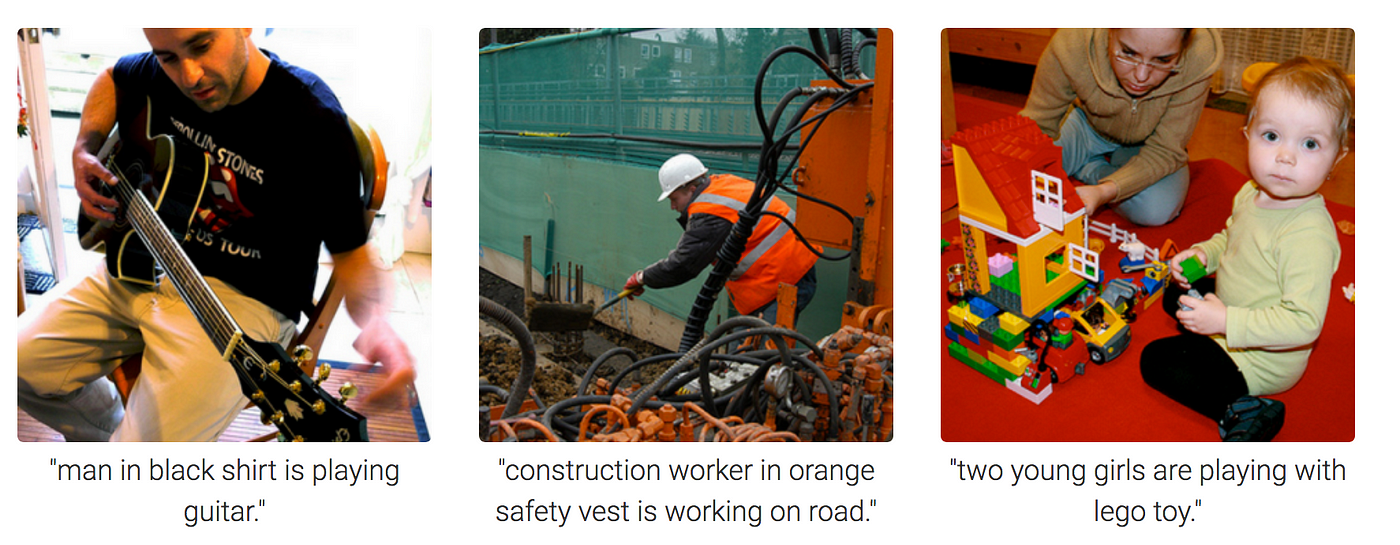
\includegraphics[scale=0.2]{img/image_captioning.png}
    \caption{Image captioning on various image prompts. } 
    \label{fig:image_captioning}
  \end{figure}

\section{Autoregressive Models} 

\subsection{NADE}

Introduced in 2011 as alternative to RBMs. 

\subsection{PixelRNN} 


\subsection{PixelCNN}  



\bibliographystyle{alpha}
\bibliography{./bibfile}
\end{document}

